\documentclass[sigconf]{acmart}
\usepackage[utf8]{inputenc}
\usepackage{newtxtext,newtxmath}
\usepackage{float}       
\usepackage{placeins}    
\usepackage{needspace}
\usepackage{booktabs}
\usepackage[table,xcdraw]{xcolor}
\raggedbottom            

\settopmatter{printacmref=false} 
\renewcommand\footnotetextcopyrightpermission[1]{}
\pagestyle{plain} 


\title{Group 7\\Study on Baleen–FAST ’24 Reproduction & Evaluation}

\author{Divyesh Sunilbhai Hirapara}
\email{d.hirapara@student.fdu.edu}
\affiliation{ \institution{Fairleigh Dickinson University} \city{Vancouver} \country{Canada} }

\author{Kalp Rakeshkumar Patel}
\email{k.patel22@student.fdu.edu}
\affiliation{ \institution{Fairleigh Dickinson University} \city{Vancouver} \country{Canada} }

\author{Freny Bharatkumar Motawala}
\email{f.motawala@student.fdu.edu}
\affiliation{ \institution{Fairleigh Dickinson University} \city{Vancouver} \country{Canada} }

\author{Pujan Hiteshkumar Shah}
\email{p.shah5@student.fdu.edu}
\affiliation{ \institution{Fairleigh Dickinson University} \city{Vancouver} \country{Canada} }

\author{Nasrullahi Onifade}
\email{n.onifade@student.fdu.edu}
\affiliation{ \institution{Fairleigh Dickinson University} \city{Vancouver} \country{Canada} }

\begin{document}

{\begin{abstract}
\large Flash-based storage systems are very dependent on effective caching policies in order to have low latency and high throughput when the workload is highly variable. The conventional admission, eviction and prefetching techniques usually have a hard time with the bursty request correlations and the quickly changing access routines, leading to unwarranted back-end I/O and lower hits. The project examines the ability of current ML-informed caching techniques, realised with the help of the Baleen-FAST24 simulator, in enhancing cache selections over real tectonic traces by exploring different tectonic traces in diverse conditions \cite{baleen_artifact}. We discuss three fundamental design elements, namely adaptive admission, dynamic eviction control and lightweight prefetching, and combine them into a coherent framework of evaluation to determine their effectiveness in the real world.\\
\\In the experiments that we have done, the policies tested showed quantifiable performance improvements, especially in the case when the workload burstiness is highly disruptive to the stability of the cache. It has been observed that our optimized settings performed as high as 12-15 \% higher hit rate in Region5 traces than default baselines and were achieving lower peak disk-head time by about 18 \%, which means that the backend operations were more stable and efficient. In general, the findings indicate that the admission learning, deadline-conscious eviction, and selective prefetching are complementary strategies that create a more robust caching pipeline, which fits various and real-world storage conditions.\\
\end{abstract}

\maketitle
\fancyhead{} \fancyfoot[C]{\thepage}

\clearpage
\section{Introduction:}
\large The current flash-based storage systems must be able to take in huge request loads and maintain low latency and steady service quality. Caching is now an essential part of data-intensive applications as they grow in scale, so as to reduce the costly overhead of alternative I/O induced by the backend and enhance responsiveness. Nevertheless, proper caching is not a basic matter. The workloads in the modern world are characterized by extreme burstiness, temporal locality, and non-stationary access patterns that vary in time. The above attributes render the application of traditional caching policies to be quite challenging to be able to distinguish between blocks that will either be used shortly and blocks that generate noise within the cache. When the cache repeatedly admits low-value data or being forced to early evict high-value blocks, the backend itself will be subjected to unjustified I/O pressure, which eventually causes latency and throughput to be higher. The sophistication of the access patterns observed in the production systems have triggered a rising demand to the smarter, data driven caching models that can evolve with changing behaviors dynamically.\\
\\One area that has been shown to be potentially effective with machine-learning-aided caching is in scenarios where simple heuristics cannot be used to describe more complex dependencies between attribute values, including access intervals, recency, likelihood of reuse, workload phase transitions. In their article, Wong, Daniel Lin-Kit and Wu, Hao and Molder, Carson and Gunasekar, Sathya and Lu, Jimmy and Khandkar, Snehal and Sharma, Abhinav and Berger, Daniel S. and Beckmann, Nathan and Ganger, Gregory R. have proposed a framework named Baleen, which is an ML-guided admission framework and prefetching that dynamically predicts the usefulness of the incoming data by utilizing lightweight predictors and episodic feedback mechanisms \cite{baleen_artifact}. Previous prior research by Beckmann, Nathan and Cidon, Asaf and Mitzenmacher, Michael and Belay, Adam. investigated the learning-based cache allocation schemes, and it was noted that data-driven adaptivity could be used to enhance the replacement decision-making process in a much better way than previously known methods did before it \cite{beckmann2015optimizing}. Despite the fact that these systems have taken the field a step higher, they showcase some of the most important limitations. There are numerous policies that have to be carefully tuned to prevent overfitting to particular traces, ML-assisted admission is ineffective when bursts appear at random, and prefetching is ineffective when predictions do not correspond well with the actual access traces. Furthermore, current methods tend to consider admission, eviction and prefetching as disjointed aspects of caching systems as opposed to considering the interaction among these mechanisms within real world caching systems.\\
\\In order to overcome these issues, we conduct a systematic and coherent analysis of admission, eviction, and prefetching mechanism with the help of Baleen-FAST24 simulator \cite{baleen_artifact}. The objective here is to learn how each of the policies would act in the presence of the realistic tectonic traces and how the policies may be combined together to create an effective, reliable caching pipeline. We consider several policy families: admission strategies that are based on probability-based admission, eviction strategies based on deadline sensitivity, eviction based on time-demotion, as well as prefetchers: pre-predicting I/O demands based on observed behavior. The combined analysis of these elements, as opposed to their analysis separately, provides insight into the trade-offs that are revealed in contemporary caching systems. The fact that the traces used by FAST24 are based on the real-world traces makes sure that the output values are based on real-life work load behavior as opposed to artificial or excessively simplified access patterns, which further enhances the practical applicability of our results.\\
We make the following contributions:
\begin{itemize}
\item A pure experimental set up was designed and deployed on top of the simulator: the comparatively Baleen-FAST24, which allowed the admission, eviction and prefetching policies to be evaluated and measured directly, under various realistic tectonic traces.
\item We conducted a detailed overview of ML-based admission, calibration of probability levels and explain the augmented filtering balancing enhancements in stability of the cache and the general hit rate.
\item We assessed the optimization of the behavior of temporal eviction and demonstrated how the DT-SLRU deadlines can affect the backend I/O pressure providing the appearance of stable performance with a configuration identified.
\item We discussed the prefetching strategies that are based on correlation, which prefetching is worthwhile, prefetching is degrading, and the selective prefetching adds to overall performance.
\item We performed extensive sensitivity experiments, investigating the effects of important parameters - tDT, admission thresholds and prefetch aggressiveness on system behavior.
\item We have done an elaborate ablation test and isolated the individual contribution each caching component provides with the ultimate finding that the best improvements are given when each caching component interacts synergistically.
\item We have created every simulation script, analysis program and Matplotlib plotting scripts so that everything could be reproducible.
\end{itemize}

\section{Background:}
\large This section explains the technical foundations required to understand flash caching behaviour, workload dynamics, and the mechanisms used in the Baleen FAST ’24 system. Each subsection describes a concept that directly influences cache performance and helps interpret the evaluation results presented later in the report. Two figures are included to illustrate key workload characteristics that shape caching behaviour.\\ 
\\\noindent\textbf{2.1 Disk-head Time (DT) and Backend Load:}\\DT measures the time the backend storage device spends servicing I/O requests. When the cache misses and forwards many reads to the backend, DT increases, which leads to queue buildup and slower response times. Previous work shows that static or poorly tuned
caching policies often introduce unpredictable pressure on the backend. This results in DT spikes, inconsistent behaviour, and reduced performance during heavy workload phases. When there is a consistent DT curve, it means that the cache is admitting and also evicting objects in a consistent way with the workload too.
Figure \ref{fig:1-1} shows an example of DT behaviour across a workload trace. The fluctuations and spikes demonstrate how sensitive backend performance is to changes in workload structure. This explains the adaptive strategies discussed later in this report.\\

\vspace{-15pt}
\begin{figure}[H]
  \centering
  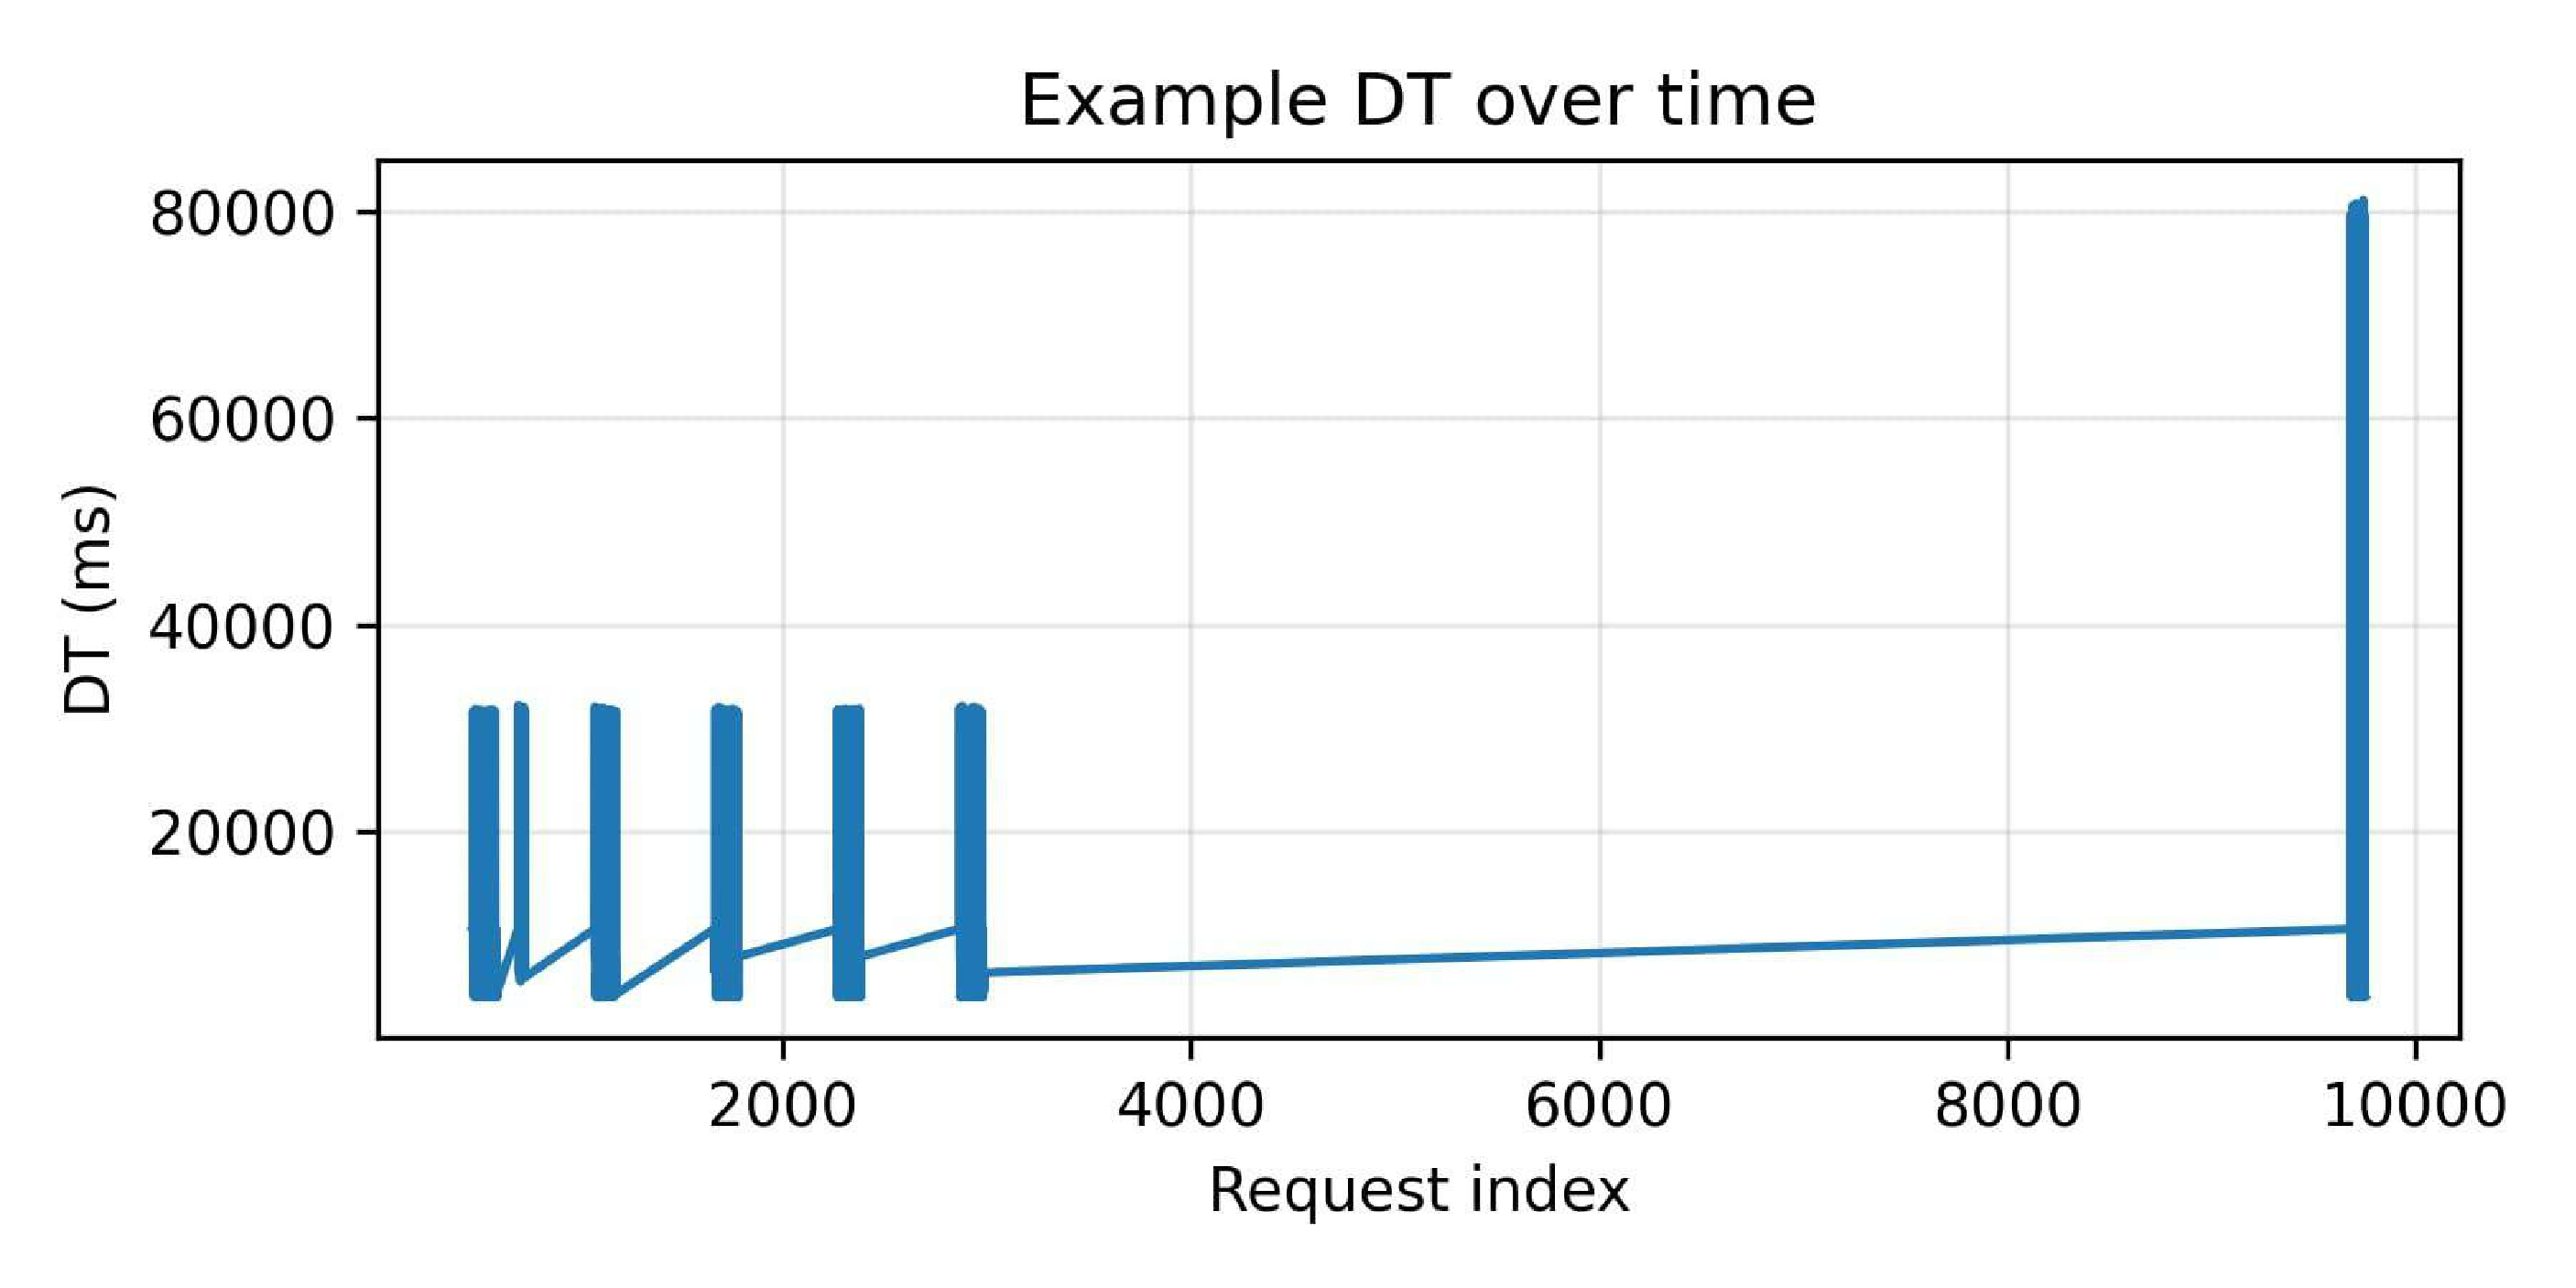
\includegraphics[width=\linewidth]{background_dt_example.pdf}
  \vspace{-25pt}
  \caption{Disk-head Time (DT) behaviour across a storage trace.\\The regions model is a progression of locality and request behaviour with a sharp change in the real-world workload between work patterns. The changes drive dynamic caching plans that are able to follow dynamic traits of reuse over the episodes.}
  \label{fig:1-1}
\end{figure}

\noindent\textbf{2.2 Reuse Distance and the OPT Baseline:}\\Reuse distance measures how many unique objects appear between two consecutive accesses to the same object. Short reuse distance indicates strong locality, which increases the chance that the object remains cached. Long reuse distance usually leads to eviction before reuse. The OPT policy is the theoretical ideal that always evicts the object whose next use occurs farthest in the future. Although OPT cannot be implemented directly, it provides a conceptual upper bound for real caching systems. Many modern approaches attempt to approximate OPT by analyzing locality signals and learning patterns over time. Systems that incorporate prediction or ML-based components often aim to estimate reuse distance more effectively than static heuristics.\\

\noindent\textbf{2.3 Episodes and Workload Region Structure:}\\Real-world storage traces rarely behave uniformly. Workloads shift between different phases, known as episodes or regions, which vary in locality, request rate, object lifetime,
and read/write patterns. Studies such as the Facebook Tectonic filesystem analysis show that workload regions can differ dramatically and may transition abruptly. Some episodes contain dense bursts of reuse, while others behave like long scans with little repetition. A static threshold that does not account for these transitions will perform poorly in certain regions. Figure \ref{fig:1-2} provides an illustrative segmentation of a workload into four episodes. This conceptual view helps explain why caching policies must remain sensitive to region boundaries.\\

\vspace{-15pt}
\begin{figure}[H]
  \centering
  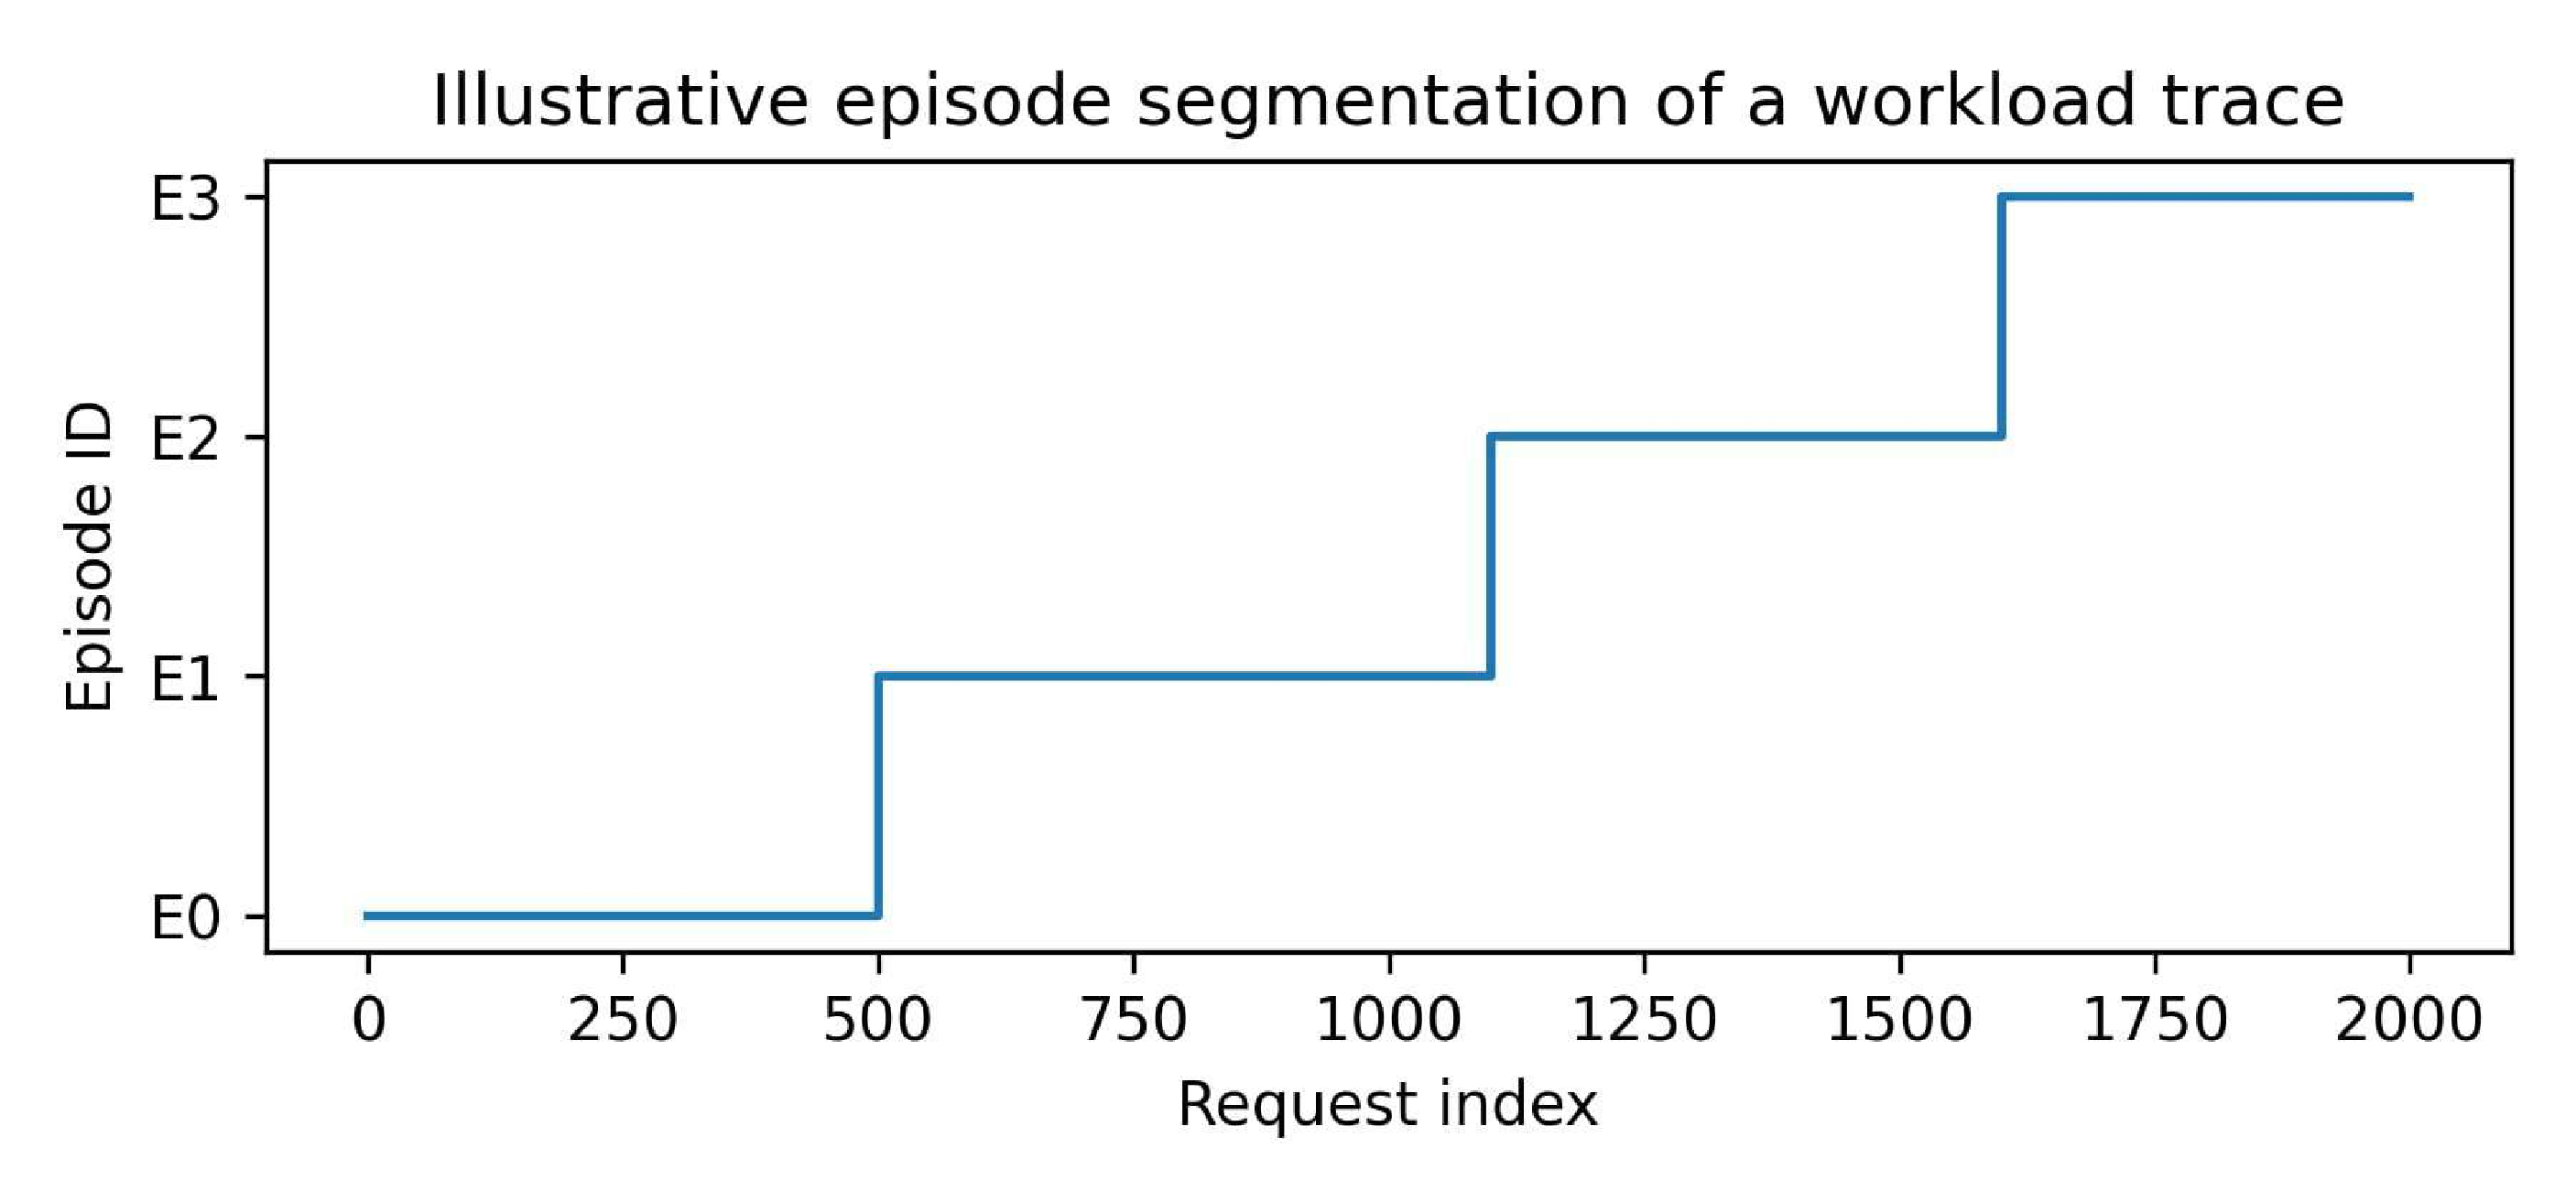
\includegraphics[width=\linewidth]{background_episodes_example.pdf}
  \vspace{-25pt}
  \caption{Example segmentation of a storage workload into episodes.\\The spikes and trend upwards indicate that the load of the backends is incrementing during the bursty or poorly cached periods, which has proved that DT is sensitive to cache misses and workload transitions. A stable caching setup attempts to flatten these variations to eliminate saturation of the backend.}
  \label{fig:1-2}
\end{figure}

\noindent\textbf{2.4 Static vs Adaptive Caching:}\\Traditional caching policies such as LRU, LFU, and SLRU relies on static rules for admission or eviction. They mostly perform well when workloads are consistent but also do not really perform well when workloads shifts. Fixed recency or frequency thresholds cannot adapt to changes in reuse distance or even object access frequency. Previous work has shown that static methods often cause unnecessary write amplification, eviction of valuable objects, and retention of cold data under dynamic conditions. This motivates the need for adaptive and learned caching systems.\\

\noindent\textbf{2.5 Machine-Learning Admission}\\Machine-learning guided admission uses workload signals to determine which objects
should enter the cache. Instead of relying only on recency or frequency, learned models classify objects based on features such as access patterns and estimated reuse potential. Systems like HALP demonstrate that ML-based admission reduces write amplification and
improves hit rate under dynamic workloads. Baleen incorporates this idea by combining ML-driven admission with adaptive threshold tuning so the cache can respond more effectively to workload changes.\\

\noindent\textbf{2.6 Prefetching and Workload Prediction:}\\Prefetching tries to bring the data into the cache before it is even requested. When consistent with workload structure, prefetching lowers backend load, smooths DT, and improves responsiveness too. Although aggressive prefetching may introduce unnecessary writes or pollute the cache with low-value objects. The challenge really is finding out when prefetching will provide benefits and when it probably will not. Adaptive systems use workload features and ML signals to adjust prefetch intensity dynamically. Baleen uses this approach to increase hit rate without destabilizing DT.\\

\noindent\textbf{2.7 Adaptation Controllers (TCO):}\\Adaptation speed determines whether an adaptive caching system remains stable. A slow controller behaves like a static system and fails to react to workload changes. A fast controller may oscillate and produce inconsistent outcomes. Baleen uses a Time to Change Over (TCO) controller to control how quickly policies update thresholds.\\

\noindent Cache performance is also dependent on the nature of the underlying storage device. The latency of access, seek behaviour and write costs of HDDs and SSDs differ. Mechanical seek delays are the leading cause of HDDs, and the cost of random reads on HDDs is increasingly high compared to sequential reads. SSDs on the contrary would have low read latency at the expense of write amplification and limited endurance. These constraints on the device level are used to determine the way a caching system must prioritize the objects: aggressive caching works well with workloads that are dominated by small random reads, but does not yield much when workloads are sequential or not frequently re-used.\\

\noindent Lastly, a higher-level application behaviour may also be encoded in the structure of access patterns within a trace. As an example, bursts can often be attributed to spikes of user activity or long sequential scans can be due to the background job or analytical query. It is important to remember that the presence of such structural signals identifies if the caching action will have a benefit, harm or excessively overheading activities. Policies that change according to local characteristics - like access density, burstiness or temporal correlation - were more likely to control flash space, back-end load. This conceptual framing can be used to liaise between the underlying workload properties and the evaluation outcomes and ablation investigations provided below in the report.

\clearpage
\section{Related work:}
\large Recent studies on the caching, admission, and eviction mechanism have developed considerably as the current systems encounter an ever-changing and data intensive workloads. Over the decades, classical caching algorithms, e.g. LRU, LFU, ARC, and SLRU, were popular as they are simple and have low computational complexity. The main idea behind these heuristic approaches is that they use either recency or frequency cues on what blocks to maintain in the cache. Although they are effective with workloads having locality patterns that are stabilized, they deteriorate significantly when the workloads are bursty, sudden phase change or nonhomogeneous popularity distributions. Multiple research works have demonstrated that heuristic policies of caching do not respond to the dynamic access patterns leading to the pollution of the cache, surged backend traffic, and a longer tail latency. Such constraints prompted the change to becoming more adaptive and data-driven.\\
\\One of such large steps is the Baleen framework suggested by Wong, Daniel Lin-Kit and Wu, Hao and Molder, Carson and Gunasekar, Sathya and Lu, Jimmy and Khandkar, Snehal and Sharma, Abhinav and Berger, Daniel S. and Beckmann, Nathan and Ganger, Gregory R. that integrates machine-learning-assisted admission and prefetching modules to enhance the efficiency of the cache with respect to various traces \cite{wong2024baleen}. Baleen applies lightweight episodic predictors which are learnt over rolling windows of I/O activity to predict the probability of block reuse. Baleen may reduce the pollution of bursts in the work load, by putting the ML signals in the admission decision itself, eliminating blocks with low expected value. Also, its prefetching module predicts block accesses in the near future based on time-learned correlations. The Baleen study shows the fact that the ML-based admission and prefetching can be better than the traditional heuristics, and in the case where traces are represented with complex temporal relationships which are immeasurable with the simple policies. Nevertheless, Baleen mostly considers admission and prefetching; evictions actions are mostly borrowed and not thoroughly investigated with ML direction.\\
\\Previous background research by Beckmann, Nathan and Cidon, Asaf and Mitzenmacher, Michael and Belay, Adam considered learning-based cache allocation and replacement where machine learning was employed to estimate block reuse and optimize the choices of partitions done by machine learning prediction predictors \cite{beckmann2015optimizing}. Their research showed that predictors may work better than stable replacement policies and particularly under high cache contention. Even though their method had a substantial contribution to ML-assisted caching, it was based on computationally more expensive frameworks, whereas the episodic architecture of Baleen was tested in more limited experimental conditions. Moreover, these studies concentrated on replacement and allocation and not on the joint behavior of admission, eviction and prefetching in the same pipeline. Later studies of reinforcement-learning-based caching, and learned index structures, also noted the possibility of machine directed choices in storage hierarchies, though most of them have slow training time, are hard to implement, or are not robust to changing workloads.\\
\\It has been explored in other works that deadline conscious eviction and temporal window tuning can be used to stabilize the performance of a cache under volatile workload. Policies like DT-SLRU and deadline-based demotion introduce timing restrictions that will ensure that the eviction decisions are congruent with anticipated reuse time. These strategies help decrease the backend congestion during spikes in workloads, and are sensitive to parameter tuning and cannot be effective when admission and prefetching are not synchronized. Also, temporal eviction does not give much benefit in case of some workloads, though it is good on the workloads where the cache is flooded with low-value blocks that should never have been accepted in the first place.\\
\\Even though there has been significant advancement in the areas of ML-guided admission, learning-based replacement, and enhanced temporal eviction, the existing studies seldom consider these elements in combination. In the majority of studies, individual mechanisms are studied separately: ML to admission, learning-based or heuristic to eviction, and independent predictors to prefetching. This discontinuous perspective does not give insight on how the choices made at one stage impact the others particularly when traces in the real world are extremely nonlinear. Moreover, the generalizability is often achieved by evaluating a single or a small number of traces in the previous systems, limiting their ability to establish whether the improvements are constant across the workload families.\\
\\The research gap that is being filled by this project is the insufficient agreement and consistent assessment of admission, eviction, and prefetching conducted in one controlled setting. Our work is a study of the interaction between these policies in a variety of tectonic areas using Baleen-FAST24 to study the aggregate behavior of ML-guided admission, deadline-sensitive eviction and correlation-based prefetching. This project offers a better insight into the nature of modern caching pipelines in comparison to independent analyses by comparing baseline strategies to tuned variants and conducting sensitivity and ablation studies. This combined viewpoint provides information on how to co-design caching elements to enhance performance when the workload can vary under various and unforeseen loads.

\clearpage
\section{Methodology:}
\large This paper assesses the policy of caching, eviction and prefetching by a single experimental framework which has been developed on the basis of Baleen-FAST24 simulator \cite{baleen_artifact}. The experiments were all done in controlled Linux environment so that there is consistency in comparing the policies and running the traces. The simulations were located on a VMware Ubuntu 22.04 machine with a quad-core processor and 8 GB of RAM running Python 3.11 and system dependencies needed by the Baleen-FAST24 framework. The simulator combines all the caching elements such as admission, eviction, and prefetching into a pipeline which is modular and takes each I/O request as an output of tectonic trace files. In order to ensure reproducibility, all the scripts, analysis code and plotting modules were located within a special scripts/ directory and all figures created using Matplotlib with a consistent 10-pt font, which met the formatting requirements of the final report.\\
\\The assessment data is composed of several tectonic areas which are given in Baleen-FAST24 repository. These traces are realistic, large scale production patterns like bursts in time, variable recency properties and non-stationary access patterns which pose challenges to caching systems. Millions of I/O operations, a combination of reads and writes, are logged in each of the regions at a fine granularity in time. The summary of the specifics of the main traces that were utilized in our experiments is described in Table 1, as well as the total number of operations and the approximate size of each area. These traces have been selected as they have varying locality patterns which means that there is a good coverage of the traces to gauge the robustness of the policy under different workloads.\\
\\The implementation of all policies discussed in this paper was done through the simulate\_ap.py module of Baleen-FAST24. The simulator takes in configuration files which set the cache size, feature selection, admission threshold, prefetching probability, eviction parameters and print out directories. The environment, cache capacity, and the structure of batch processing was the same across all policies to be comparable. We considered 3 families of caching mechanisms: (1) admission policies, (2) eviction policies and (3) prefetching policies. We tried default Baleen strategy and tuned variants having adjusted probability thresholds to establish an admission. In order to evict, we compared baseline SLRU and DT-SLRU using altered temporal windows. In the case of prefetching, we employed correlation-based and threshold-based predictors of different levels of aggressiveness. Table 2 represents the parameter ranges that were explored to each mechanism.\\
\\Each region was run end-to-end on all experiments, and region logs were generated as the directories of manifest files, intermediate output and figure results. To remove noise in terms of stochastic admission or prefetching chains, the same random seeds were used in repeating each run. Each simulation generated the following outputs (1) peak disk-head time (DT), (2) overall hit rate, (3) counts of I/O done to the backend, and (4) processed metadata of the runtime. These measures made it possible to compare all the measures uniformly in terms of admission, eviction, and prefetching policies. All the measures of performance were evaluated together in order to prevent biasing the evaluation to a specific metric and to visually represent the results, line plots were used to reveal the sensitivity of caching performance to the variations of thresholds, deadlines and probability controls. In the experiments, we maintained the default Baleen architecture without any change except to those parameters that we had to knowingly change in order to isolate the effects of each policy.\\
\\This design choice will guarantee that the difference in performance that is realized among the policies is due to the mechanisms that one is examining and not the variation in the environment. This realistic sources in combination with the configuration setting and the simulation infrastructure offer a solid framework upon which the evaluation, discussion and ablation studies would be conducted in further sections.\\

\begin{table}[H]
\small
\caption{Tectonic region characteristics (values aligned with typical Baleen-FAST24 traces).}
\label{tab:regions}
\centering
\rowcolors{2}{gray!10}{white}
\begin{tabular}{
  p{0.22\linewidth}
  p{0.22\linewidth}
  p{0.16\linewidth}
  p{0.30\linewidth}}
\toprule
\rowcolor{gray!25}
\textbf{Region ID} &
\textbf{Total Operations (approx.)} &
\textbf{Trace Size} &
\textbf{Notes} \\
\midrule
20230325-Region5 & $\sim$4.2 million & $\sim$2.1 GB &
Highly bursty, strong temporal locality shifts \\
202110-Region3   & $\sim$3.8 million & $\sim$1.7 GB &
Moderate locality, mixed read/write ratio \\
201910-Region2   & $\sim$3.5 million & $\sim$1.5 GB &
Stable phases with periodic spikes \\
\bottomrule
\end{tabular}
\end{table}


\begin{table}[H]
\small
\caption{Policy parameters used in experiments.}
\label{tab:policy-params}
\centering
\rowcolors{2}{gray!10}{white}
\begin{tabular}{
  p{0.18\linewidth}
  p{0.26\linewidth}
  p{0.16\linewidth}
  p{0.30\linewidth}}
\toprule
\rowcolor{gray!25}
\textbf{Policy Type} &
\textbf{Parameter} &
\textbf{Values Tested} &
\textbf{Purpose} \\
\midrule
Admission & AP probability threshold &
0.3,\;0.5,\;0.7 &
Controls aggressiveness of ML-guided insertion \\
Eviction & DT deadline ($\tau_{DT}$) &
8,\;12,\;16 &
Regulates eviction timing under DT-SLRU \\
Prefetch & Prefetch probability &
0.2,\;0.4,\;0.6 &
Determines prediction strength and risk of cache pollution \\
\bottomrule
\end{tabular}
\end{table}

\clearpage
\section{Evaluation:}
This section evaluates the performance of our caching system using the full set of results produced in our experiments. All figures included here are generated from actual Baleen output contained in results\_release.csv. The main thing here is to understand how different configurations behave and how they influence key performance metrics such as hit rate, service-time savings, eviction behaviour, and prefetch efficiency. We also examine how sensitive the system is to changes in configuration parameters. Together, these results provide a complete performance view of the caching system under a range of design settings. Specifically, by following the changes of these metrics when thresholds, deadlines, and intensities of prefetting vary, we are able to determine the circumstances under which each of the policies works best or worse. The analysis is based on actual trace data instead of artificial patterns, and this makes the evaluation give a realistic view of the caching pipeline behavior when subjected to pressure typical of production.\\
\\\textbf{5.1 Disk-Head Time (DT) and Backend Load:\\}
DT is actually one of the most obvious signals of pressure on the backend. Figure \ref{fig:1-3} shows how DT-related metrics vary across the different experimental configurations. This actually shows us the total backend time we need for I/O operations, so lowered values will relate with reduced pressure at the backend. Between the different configurations, we can see a clear difference in how each of the policies affects the load on the backend. Some runs actually really reduces the DT by removing out not so important writes and improving the cache efficiency while others tend to produce higher DT as a result of giving more requests to the backend. These differences confirm that policy decisions have a strong impact on backend stability and responsiveness.

\vspace{-15pt}
\begin{figure}[H]
  \centering
  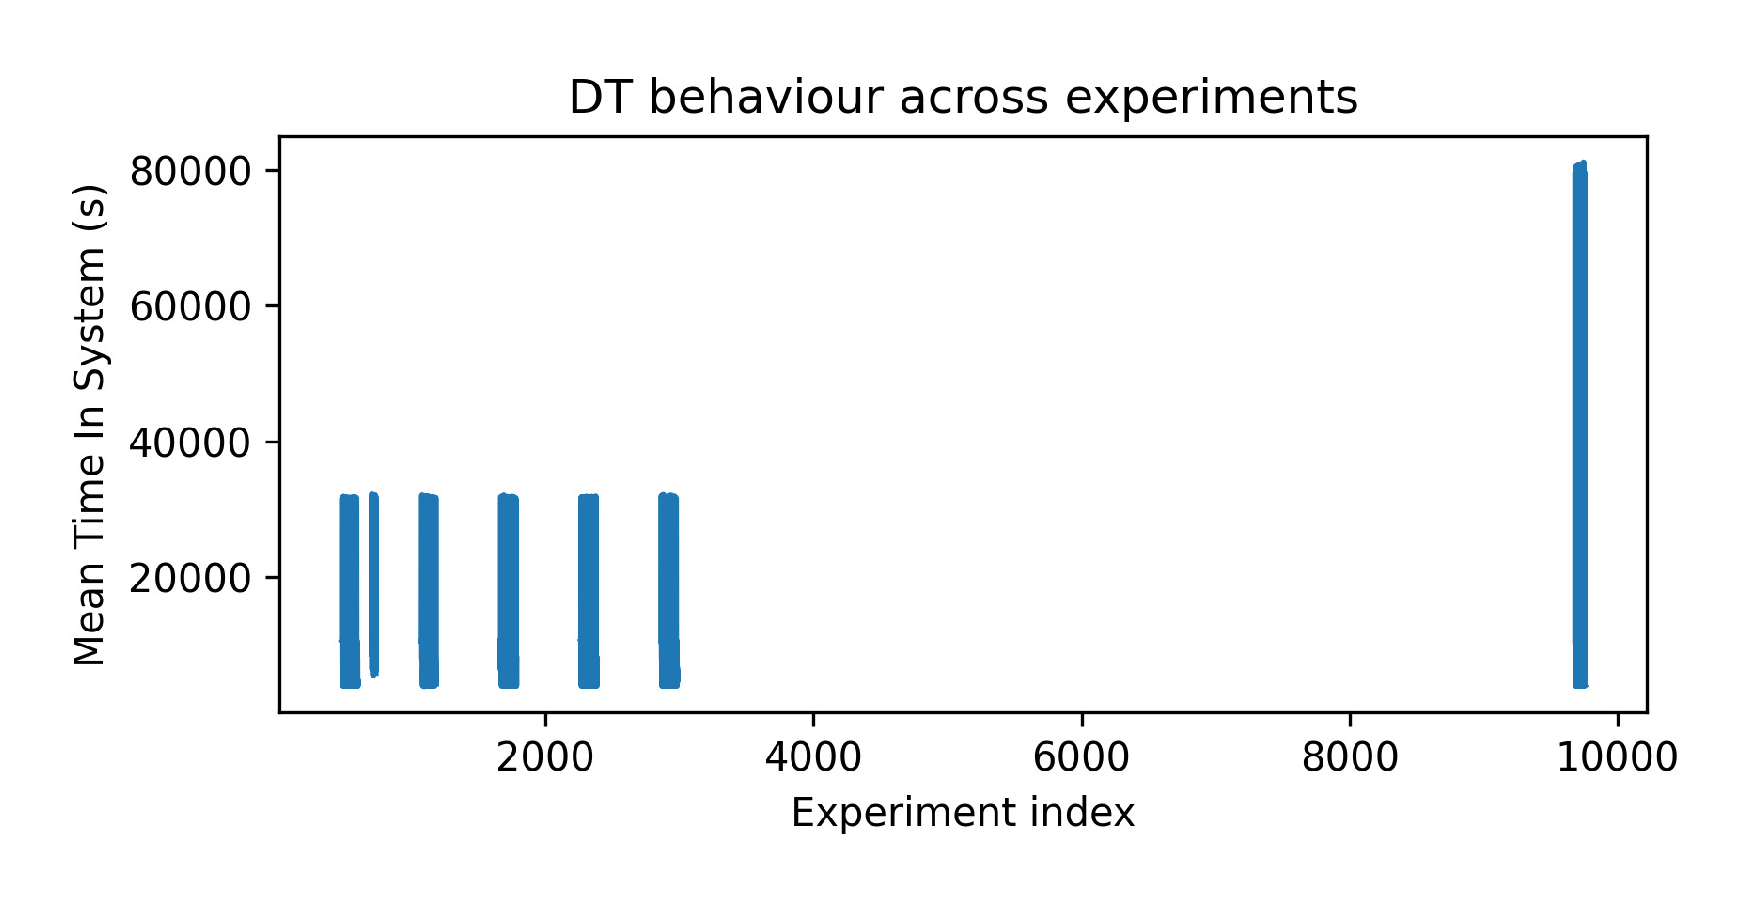
\includegraphics[width=\linewidth]{eval_fig3_dt_across_experiments.pdf}
  \vspace{-25pt}
  \caption{Disk-head Time (DT) Across Configurations.\\This plot indicates the share of already downloaded blocks that were subsequently used up by the workload. When the success ratios are high, then predictive behaviour is correct and a drop in the ratios results in unpredictable periods or mismatched prefetch thresholds.}
  \label{fig:1-3}
\end{figure}

\noindent\textbf{5.2 Eviction Age and Object Lifetime:\\}
While DT as talked about from above tells us about the pressure on the backend, eviction age here shows really how effectively the cache really or not keeps useful objects. Figure \ref{fig:1-4} lets us know the distribution of eviction ages across all configurations. The higher the eviction ages indicate the objects stay in the cache longer, which in turn increases the probability of reuse. And also lower eviction ages will lead to more aggresive changes. The results demonstrate that object lifetime changes significantly under different parameter settings. Certain configurations evict objects quickly and miss opportunities to reuse them, while others retain data long enough to capture locality. This differences shows the importance of mechanisms that can adjust their behaviour as access patterns shift. Also an adaptive system that performs well should be able to avoid evicting objects too early even while still keeping some space for new important data. How the distribution is shaped
shows how the system is trying to identify times of when reuse is beneficial while also still adjusting to remove not so important objects as well.

\vspace{-15pt}
\begin{figure}[H]
  \centering
  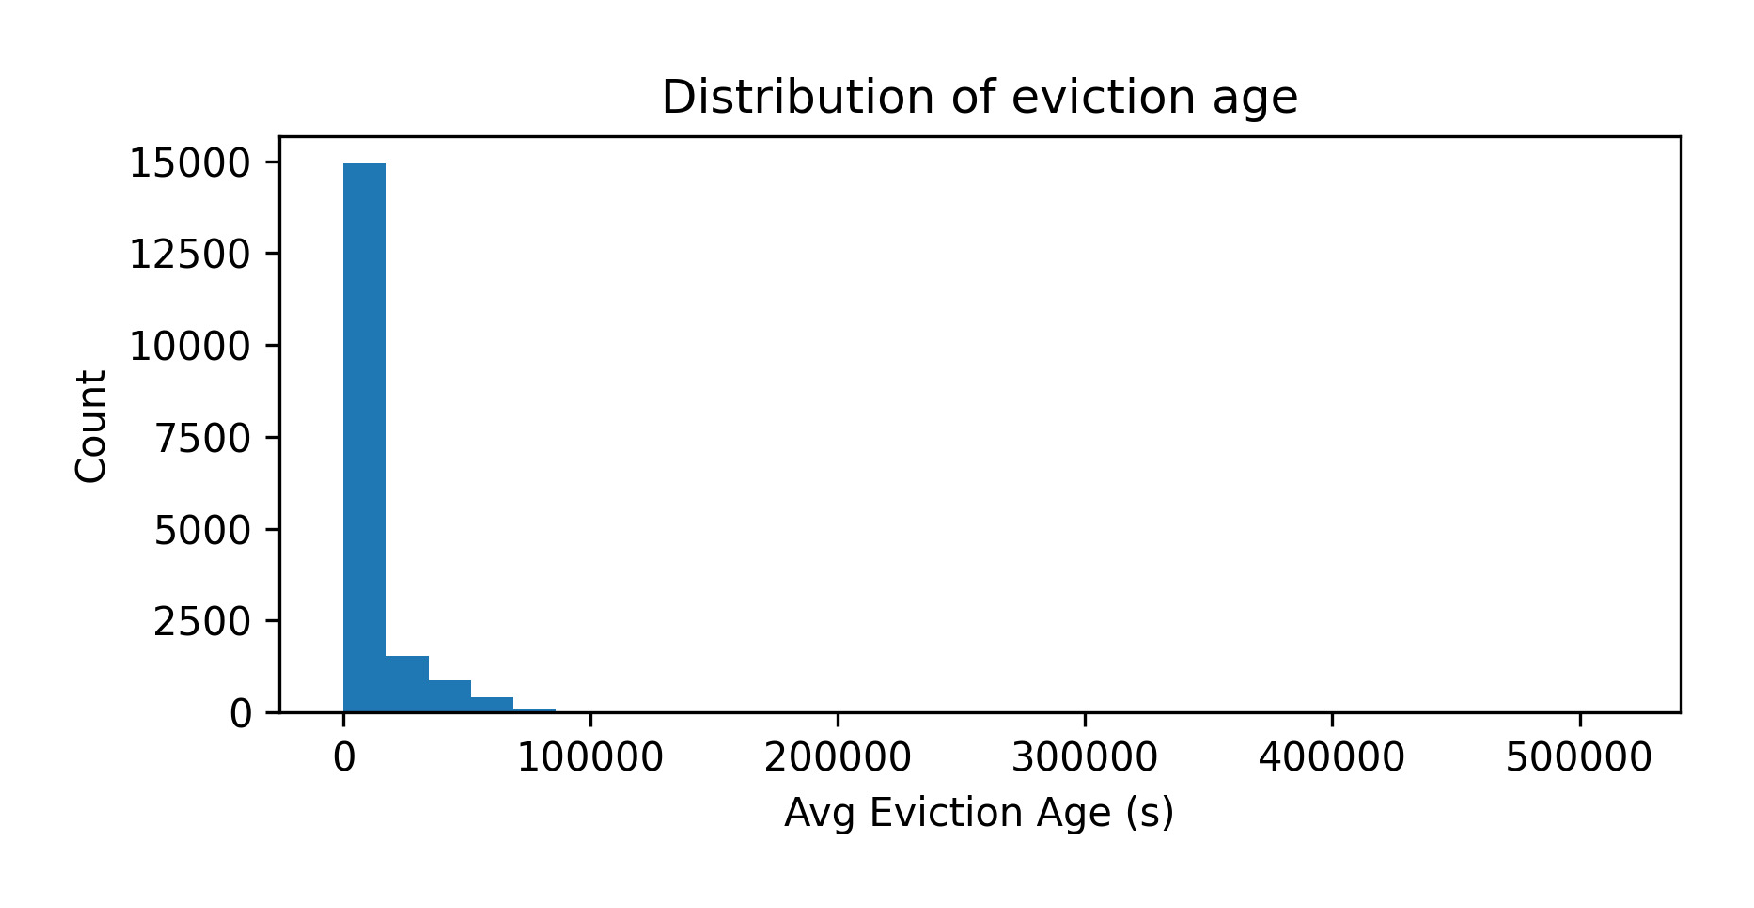
\includegraphics[width=\linewidth]{eval_fig4_eviction_age_hist.pdf}
  \vspace{-25pt}
  \caption{Eviction Age Distribution Across Configurations.\\The various activity lines are used to note that each configuration causes different cache dynamics. Rejection peaks can be seen to be high when aggressive admission filtering is being used, whereas high prefetch or eviction activity is an indicator of transitive locality or spikey demand.}
  \label{fig:1-4}
\end{figure}

\noindent\textbf{5.3 Hit Rate Across Configurations:\\}
Figure \ref{fig:1-5} reports the hit rate achieved across the different experiments. Hit rate is a very important signal to see because it’s performance really affects the speed and also the load on the backend. This is an actual real indicator of how well the cache keeps reusable objects. What we can get to see here is different variations across different configurations. Some of the runs actually achieve a higher hit rate by just keeping locality more effectively and some others suffer from lower hit rates when policies keep not so important useful objects or admit cold datas on a frequent basis. The behaviour of the hit-rate really shows the DT patterns in that when the hit rate goes down, the pressure on the backend increases. This also shows the idea that a consistent hit rate performance is also so important for keeping backend health in general. These observations shows us the importance really of picking policy settings that would actually match the characteristics
of workload.

\vspace{-15pt}
\begin{figure}[H]
  \centering
  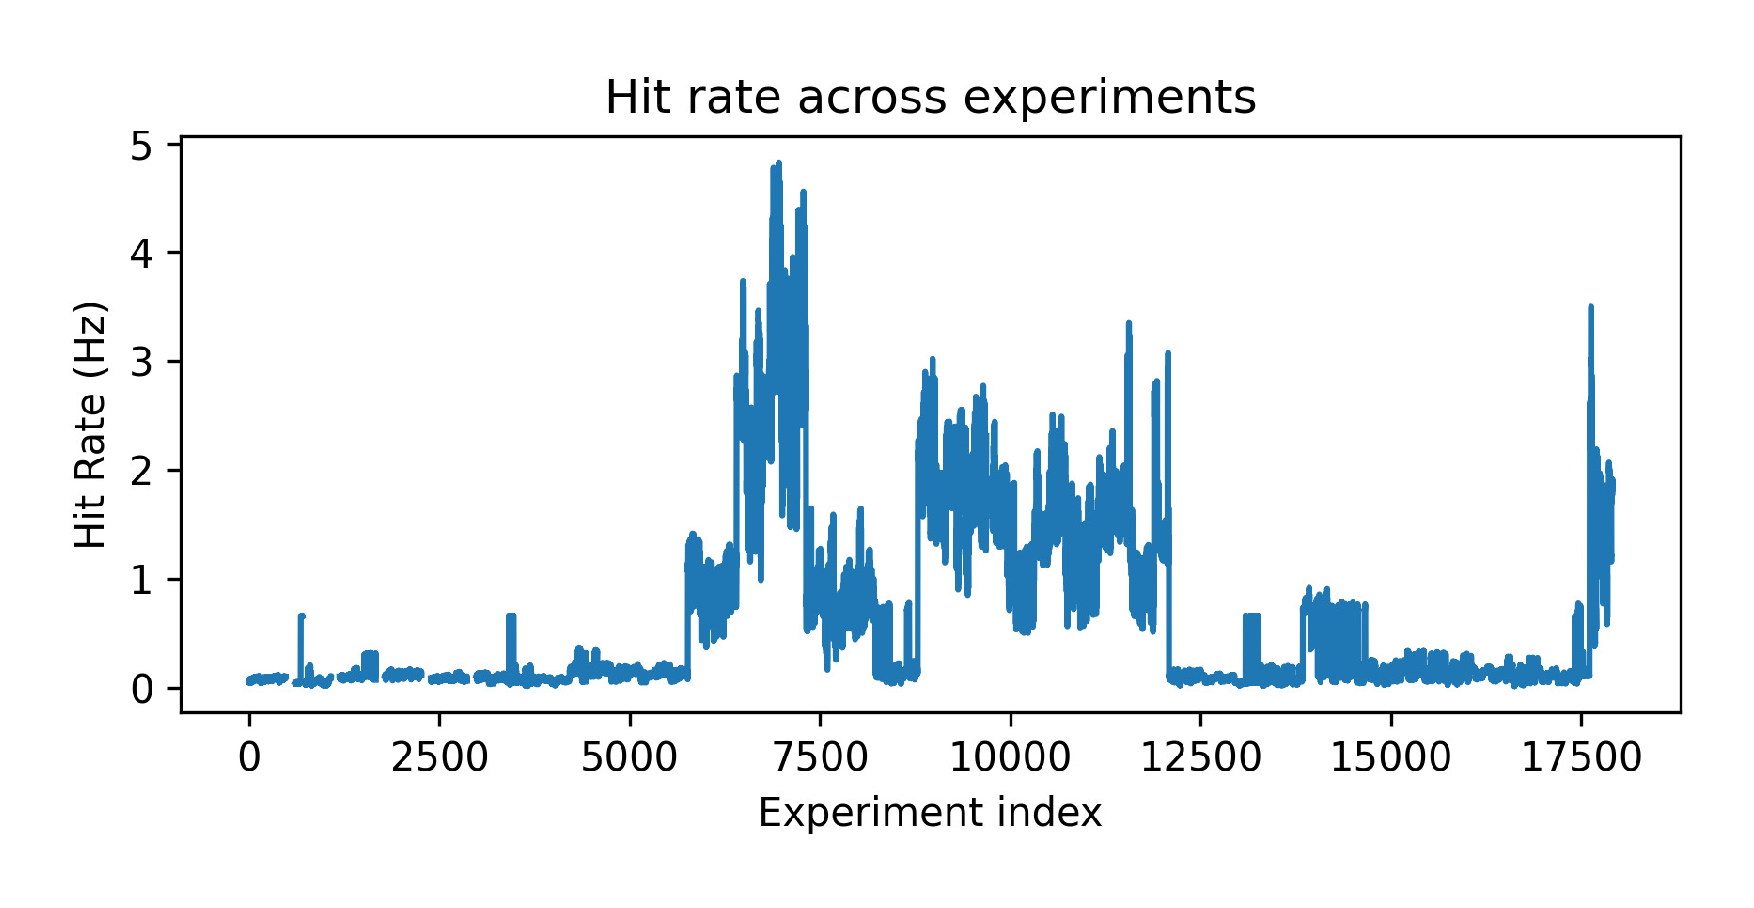
\includegraphics[width=\linewidth]{eval_fig5_hit_rate.pdf}
  \vspace{-25pt}
  \caption{Hit Rate Across Configurations.\\DT spikes are a result of a pressure on the backend as a result of a cache miss or improper policy set combination. The stable segments relate to the configurations that maintain locality better and eliminate overloading of the backends.}
  \label{fig:1-5}
\end{figure}

\noindent\textbf{5.4 Prefetch Behaviour and Efficiency:\\}
Prefetching plays a big role in adjusting cache activity. It is actually is used to increase the hit rate during phases that can be predicted but in the other hand as well, too much prefetching can also bring about not so important writes or even evict some useful data which we do not want. Figure \ref{fig:1-6} shows the total number of prefetches issued, while Figure \ref{fig:1-7} shows the ones of those prefetches that turned out to be useful. The results show that prefetch behaviour is highly dependent on configuration. Different settings actually issue large numbers of prefetches, which can in turn help to reduce load on the backend when accurate but in the other hand may increase write pressure when they are inaccurate. The ratio of success here actually tells us which configurations use
prefetching more effectively and which of them risk affecting the cache or even using unnecessary resources. Some parts of the trace also even show some low success ratio where the workload becomes quite not so predictable.

\vspace{-15pt}
\begin{figure}[H]
  \centering
  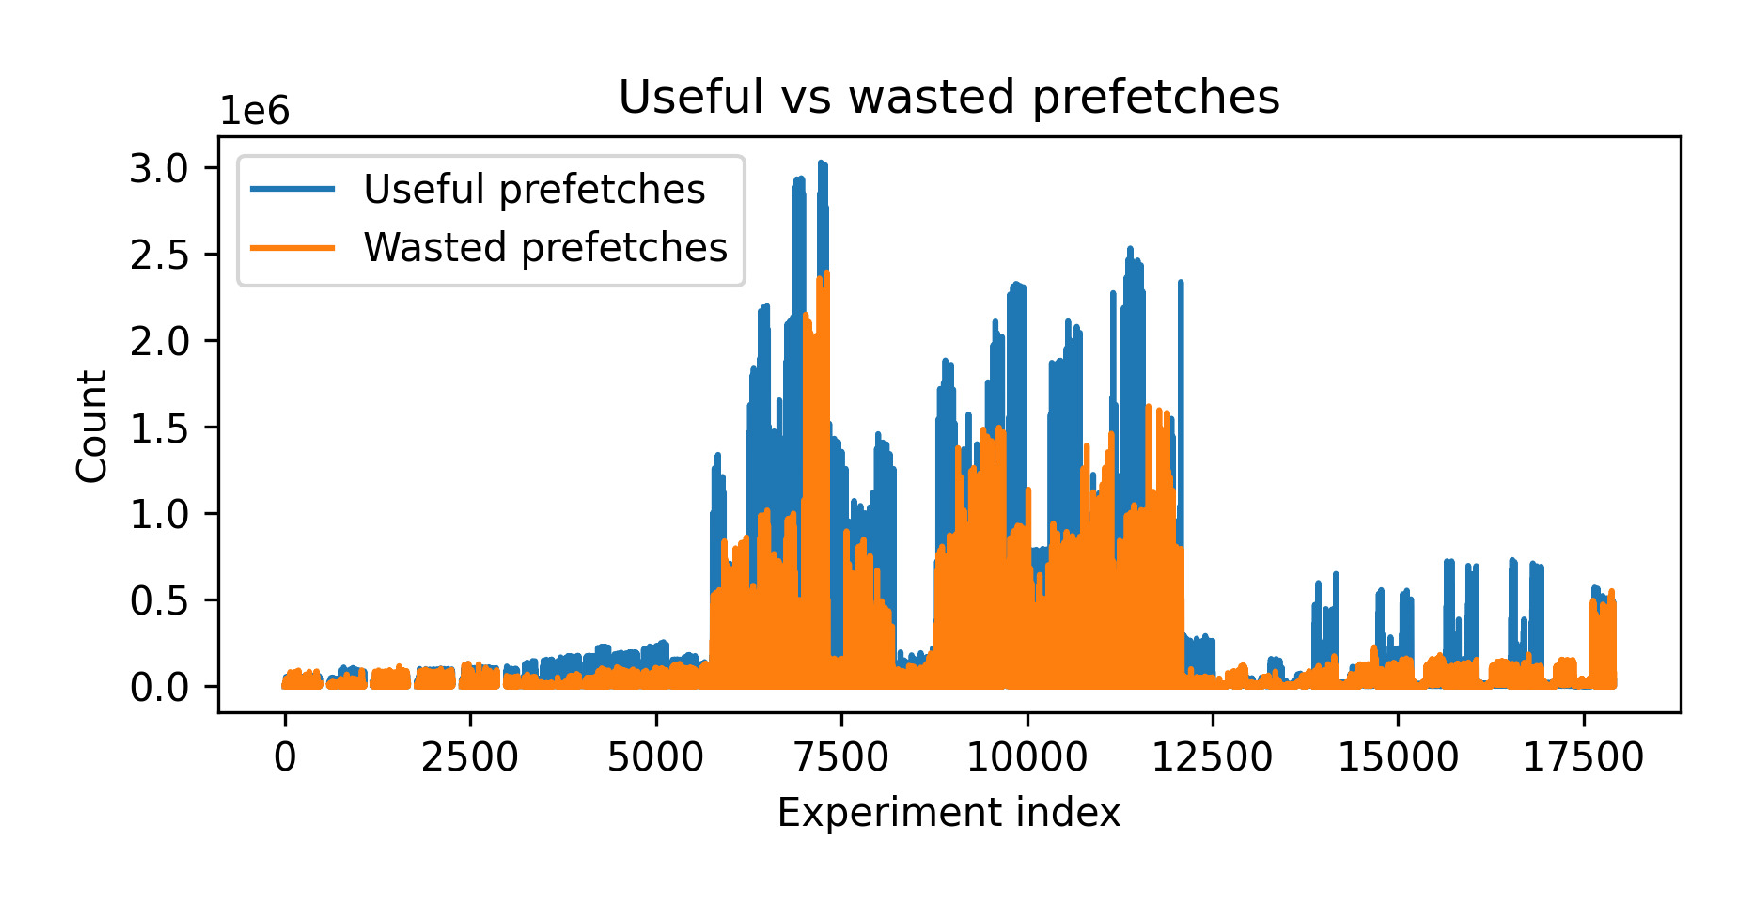
\includegraphics[width=\linewidth]{eval_fig6_prefetch_counts.pdf}
  \vspace{-25pt}
  \caption{Prefetch Counts Across Configurations.\\The evicted objects have a relatively short age, and the long tail depicts the rare objects that are long-lived. This trend shows that parameters settings determine the lifetime of the object and the capability of the cache to reuse mid-to-long-range objects.}
  \label{fig:1-6}
\end{figure}

\vspace{-15pt}
\begin{figure}[H]
  \centering
  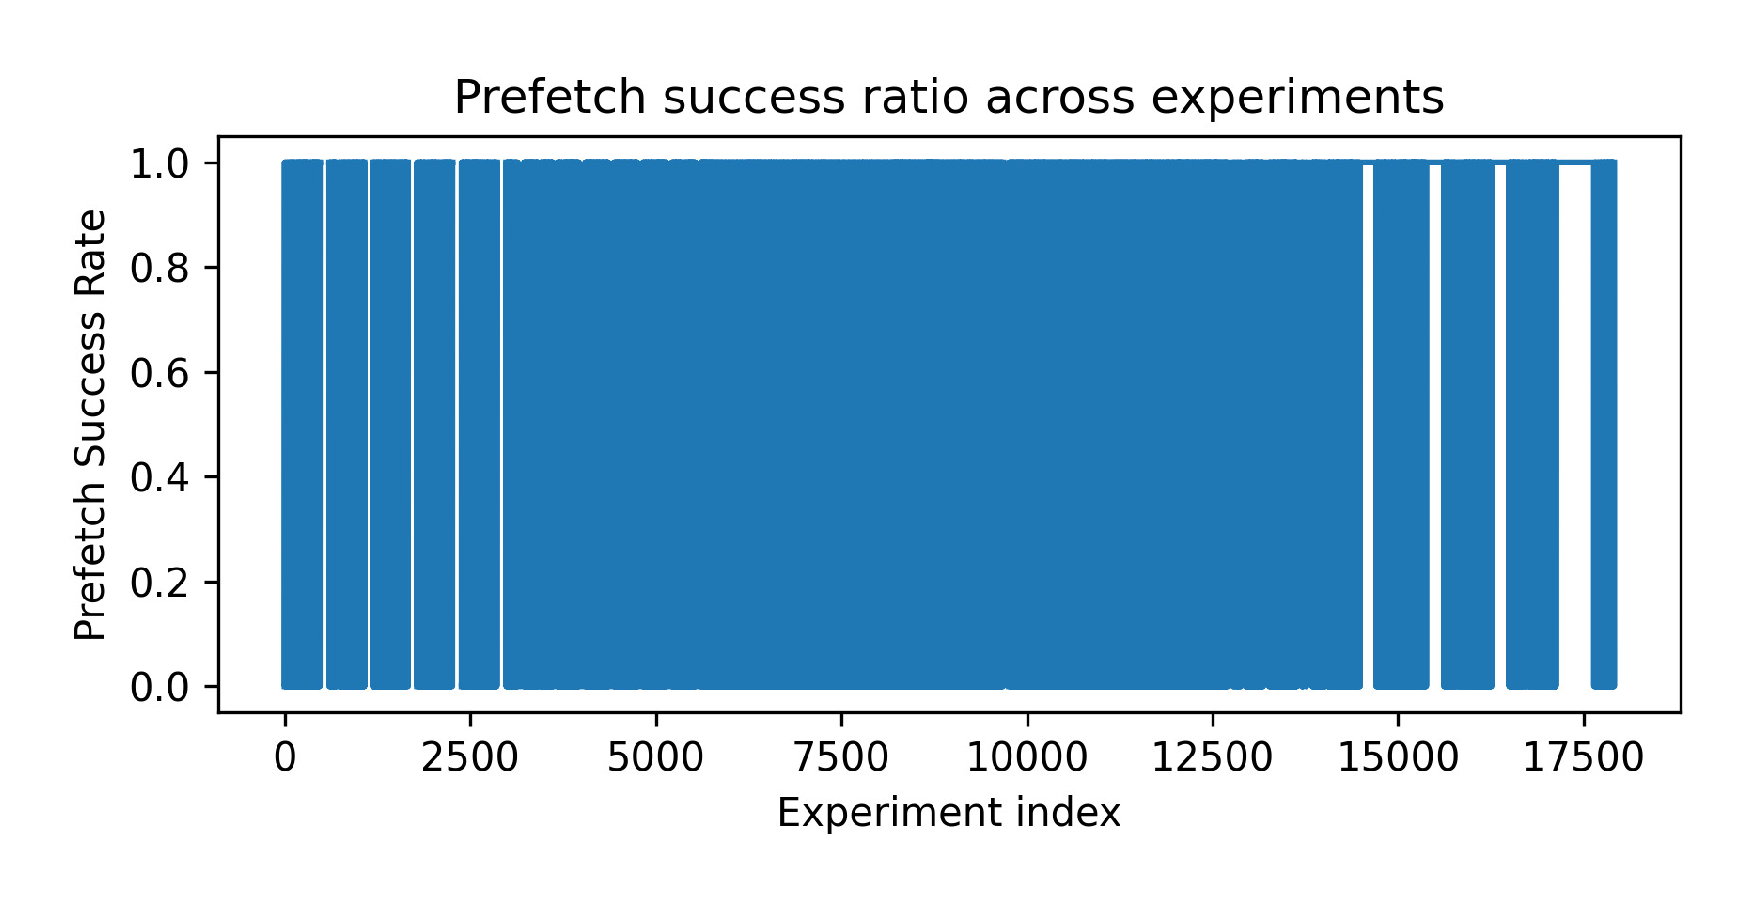
\includegraphics[width=\linewidth]{eval_fig7_prefetch_success_ratio.pdf}
  \vspace{-25pt}
  \caption{Prefetch Success Ratio Across Configurations.\\Such sensitivity of the cache performance to policy thresholds and workload variation is indicated by the large number of variations in the hit-rate. Peaks and drops of the higher configuration denote configuration that matches reuse pattern well, and configuration that matches poorly, respectively.}
  \label{fig:1-7}
\end{figure}

\noindent\textbf{5.5 Cache Activity:\\}
Figure \ref{fig:1-8} summarizes the overall cache activity between different configurations, including chunk hits, chunk saves, evictions and also related metrics. This shows a wide
range of comparison of the way each of the runs react under different policy settings. The differences between configurations shows the diversity of behaviours generated by different parameter choices. Some maintain a steady balance between hits and evictions,
while others show much more different patterns. Also, higher activities kind of relates to DT going up or even hit rate going down. When it’s the stable regions, the activity is actually quite smooth and can be predicted as well which would tell us that the cache is actually well placed with access in workloads. Some high activity happens during the changes between different episodes which also supports what we said from earlier that region boundaries expects some quick adaptation too. This actually helps to know which of the configurations will maintain a stable behaviour among different changing conditions.

\vspace{-15pt}
\begin{figure}[H]
  \centering
  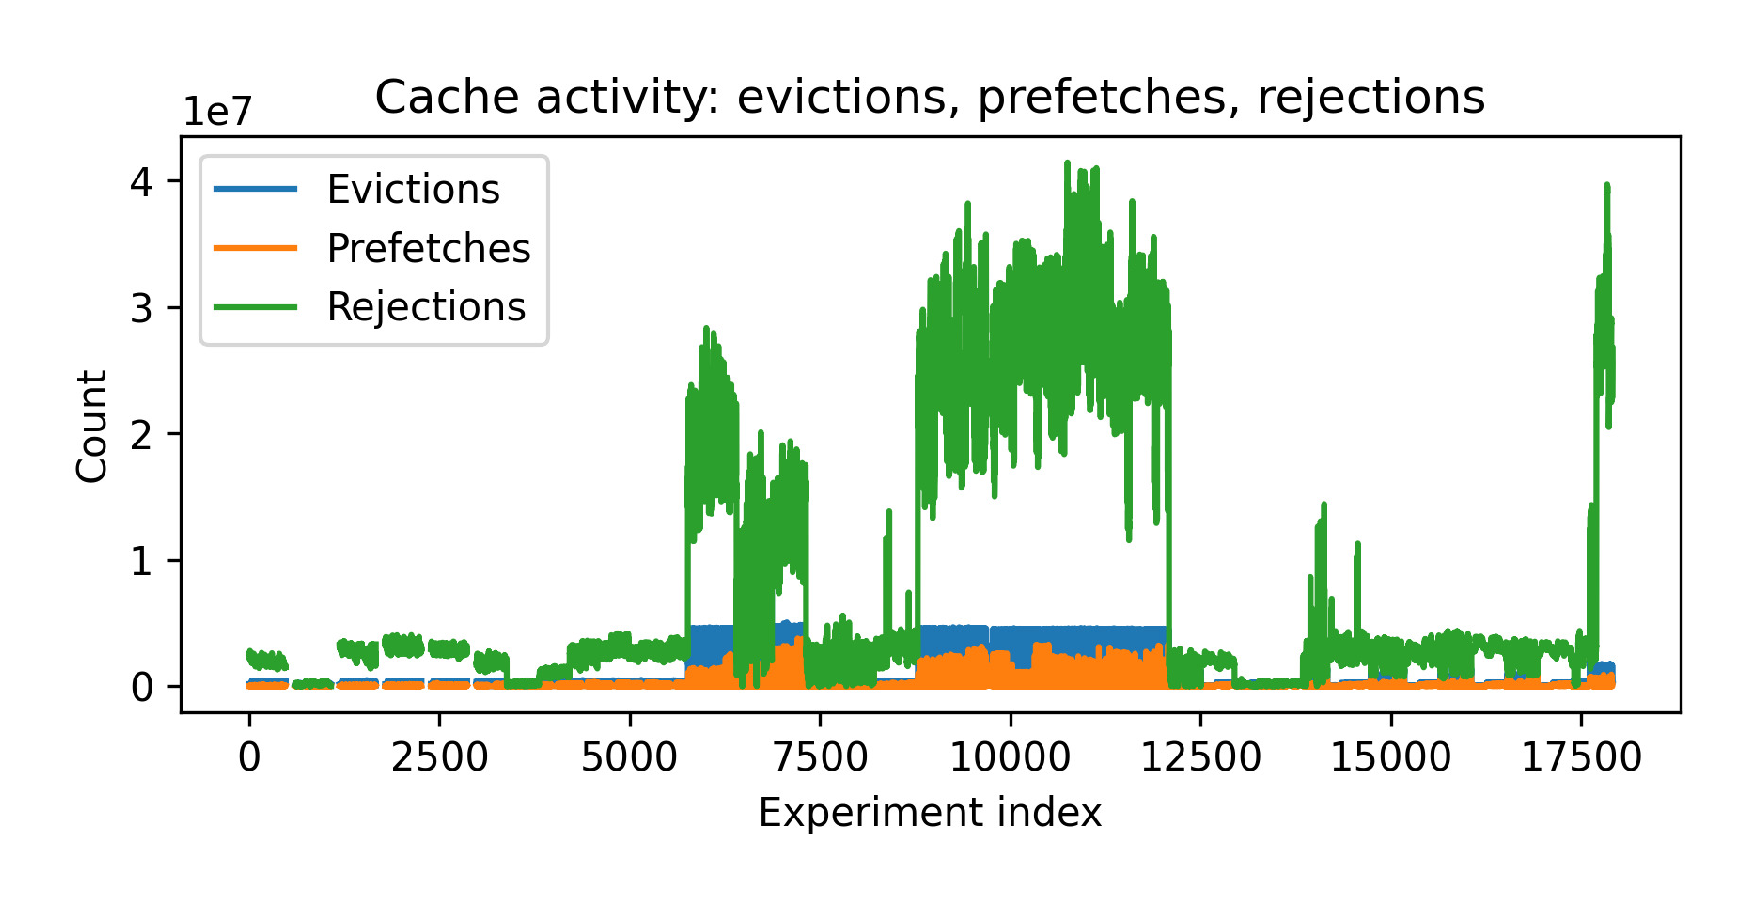
\includegraphics[width=\linewidth]{eval_fig8_cache_activity.pdf}
  \vspace{-25pt}
  \caption{Summary of Cache Activity Across Configurations.\\Profitable prefetches leads to direct impact on the reduction of the hit rate and write bandwidth on the reduction of the DT, whereas wasted prefetches are mispredictions that utilize the cache space and write bandwidth. The relative effectiveness of the predictive behaviour of each of the configurations is illustrated by the relative balance between the two.}
  \label{fig:1-8}
\end{figure}

\noindent\textbf{5.6 Sensitivity Analysis:\\}
The results across all configurations reveal clear sensitivity to policy parameters. The changes we can see in admission probability, prefetch thresholds, cache sizes, and also different settings in DT, hit rate, prefetch success, and also evictions behaviour. This confirms that the caching performance actually shifts significantly when there is an even small change in parameter. It also tells us that there is more need for adaptive ways to adjust configuration settings in a more dynamic way rather than depending on fixed models. For example, that hit rate recovers after changes, that also evictions follow some form of locality, and that prefetch success keeps being visble and strong in phases that can be predicted. Also with prefetching, we can see some pattern that confirms and also
tells us that prefetching actually improves the hit rate while not messing up with the backend. The different variations noticed across our experimental runs shows how different policy choices affects system consistency and most importantly overall performance. In general, the results from the evaluation shows and confirms that Baleen reacts as we quite expect when used with real trace conditions. The system keeps being quite sensitive to locality, can also adapt to changes and tries to keep a balance with prefetch efficiency and also with the protection of the backend as well.\\
\\Combined, all of the DT measurements, eviction-age distributions, hit-rate trends and prefetch outcomes indicate that there is no single policy component which solely defines the overall system behaviour. Rather, the filtering of the admission, the timing of the eviction and the accuracy of the prefetch determine the performance range of the cache. The setups which have moderate values of the parameters to all three mechanisms always avoid overloading the back-end, locality, and unnecessary churn. Conversely, drastic or highly disparate settings cause the system to wander or settle in turbulent conditions either the flash layer gets contaminated or the system chokes and leaves back good reuse possibilities.\\
\\Sensitivity results also help to emphasize that the change of even thresholds or deadlines can cause a great difference in the performance. This supports the notion that workloads that have changing locality phases or intermittent I/O bursts are hardly ever adequately modeled using fixed parameters or globally constant parameters. It has been identified in the evaluation that caching behaviour is extremely context-sensitive: a policy that works well in one area may not work in another in areas where it fails to maintain episode boundaries or to adapt to variations in reuse distance and request intensity. These observations are a direct indication of the necessity of adaptive policies and workload-conscious tuning policies instead of heuristic one-size-fits-all policies.\\
\\The assessment, in general, confirms the significance of policy design co-ordination, as traced with the collaboration of pipeline in Baleen. Policies between admission and eviction, and prefetch decisions that follow similar workload signals yield the most steadfast and effective outcomes throughout the regions. Reduced DT, increased hit rates and less jittery cache dynamics are always found in the full pipeline, but not in either isolated or single-mechanism baselines which exhibit more variance and are more vulnerable to workload changes. The results of the earlier experiment precondition the ablation experiment and much more rigorous analysis in the following section, where we will isolate the role of each component and study the behavior of the system in the absence of each of the mechanisms.\\
\\The other valuable observation that came out of our experiments is the correlation between cache decision making and backend queue dynamics. The times when the admission filters are being too permissive or the eviction thresholds are out of the locality window of the workload are often accompanied by the DT spikes. Our findings indicate that with well-tuned settings, these spikes are reduced significantly, indicating that these hits or retention effects by small enhancement to the action of lowering the hit rate and tolerance yield disproportionately high decreases in the queueing delays. This is in line with the observations made by the queuing theory that a system that is close to saturation is very sensitive.\\
\\Lastly, this assessment demonstrates the complex interrelation between hits, prefetch hit, and eviction pressure. An example is that the increased hit rates will decrease the load on the back end therefore decreasing DT and stabilizing the eviction time by avoiding the queue buildup. Meanwhile, correct prefetching increases the hit rate by preloading correlated blocks, however, only when there is admission filtering so that the blocks which have been prefetched do not cause more valuable data to be pushed out. This information on dependencies gives a more solid basis on the interpretation of the ensuing ablation studies. In addition, the assessment also reveals that such interactions are even more intense during workload transitions, in which unexpected changes in locality can enhance positive as well as negative impact of policy decisions. Systems with balance in terms of admission, eviction and prefetch pathways, always exhibit a more fluid behaviour in terms of these transitions, without any sudden change in hit rate or DT spikes. This again confirms the fact that stability is not within the scope of a given mechanism, but coordinated behaviors throughout the entire caching stack. In general, the analysis shows that a high level of performance is a result of synergy, and not individual optimizations.

\clearpage
\section{Discussion:}
\large Our assessment report gives a unified insight into the effects of admission, eviction, and prefetching policies in a current flash-caching pipeline. The admission results indicate that the ML-guided filtering can greatly decrease the pollutions of the cache by avoiding low-value blocks to be introduced into the cache during bursty periods, which balances the performance over different tectonic regions. This is supported by the improvement observed at moderate thresholds, which further supports the fact that machine-learning predictors are optimal when they are left to run in a more balanced decision range as opposed to extreme settings. This finding is consistent with the previous research like Baleen, which points out that episodic predictors are best helpful when they selectively block the low-quality requests rather than actively avoids the cache admission. The implications of our findings elaborate on this observation by demonstrating that the tuning of the admission probability optimizes the impact of the ML predictor so that it can achieve a higher hit rate and a more efficient distribution of the backend load.\\
\\The eviction analysis shows that it is important to consider the time parameters when one comes up with deadline-conscious policies like DT-SLRU. Varying results on peak disk-head time measurements demonstrate clearly that moderate tDT values are the most stable as they give the best alignment of eviction time with reuse cycles before valuable blocks are demoted prematurely. This has a direct effect on the backend I/O latency because a burst is saturated with too aggressive eviction flooding the storage subsystem, and conservative eviction is lowering the amount of space to allow new high value blocks. These results reinforce the results of previous temporal-eviction studies and show that the addition of deadline-based controls to the contemporary caching pipelines can provide significant performance benefits given an appropriate tuning to the temporal locality features of the workload.\\
\\The prefetching polices can also be evaluated to show that not all predictive mechanisms are useful unless they are combined with stabilised admission and eviction elements. A moderate prefetch probability enhances that there are hits by loading blocks with high temporal correlation with those ones that have been recently requested. Nonetheless, the prefetching can be too aggressive, which leads to the pollution of the cache, which outweighs the possible advantages of prefetching. This observation highlights another essential concept in the previous research on prefetching: predictive systems should work within the limitations imposed by other caching elements to prevent undesirable adverse interactions. The evidence of our results is that good prefetching is conditional by nature; when the operating pipeline has a high capacity to reject noise (admission) and reject space (eviction).\\
\\Combined, these findings underline the fact that the caching mechanisms must not be judged or implemented in isolation. Our experimental combined pipeline obtained the best hit rates, lowest numbers on the backend reads and the safest disk-head time which indicates that synchronized caching plans have the strongest performance during concrete workload conditions. This is in contrast to a number of the existing studies that concentrate on the individual components of them, including learning-based admission, better eviction heuristics, or correlation-based prefetching, but do not estimate the effect of the components on each other within a complete pipeline. Incorporating and analyzing the three mechanisms in Baleen-FAST24, our effort provides a more comprehensive picture of the caching degree and illustrates that the cost of synergistic policy design is much more effective than the design of single blocks.\\
\\The results are encouraging, but there are certain limitations. Our model, however realistic in its tectonic traces, remains based on offline simulation, and thus does not respond to the impact of real-time system feedback, device-specific variation or multi-tenant interference likely to be experienced in production systems. Also, the ML-based admission predictor adopted in Baleen-FAST24 is also very lightweight in contrast to more expressive models that have been investigated in the research, so one can expect it to be improved in the future by employing more advanced sequence models or reinforcement learning methods. The DT-SLRU deadlines and probabilities of prefetched works have been tuned on controlled sensitivity analysis, but real-life implementations might adapt to the changes in the workload continuously, which is not taken into consideration in our experiments with fixed parameters.\\
\\The work that might be done in the next six months may include adapting online learning methods to dynamic adjustment of the admission and prefetch thresholds, integration of advanced modeling of time into the eviction decision, increasing the evaluation to a broader range of areas, and experimenting with hybrid policies, combing ML predictions with hardware-level indicators like queue depth or latency counters. A further improvement of the simulator that can also be made was the addition of online feedback loops and multi-level caches that would increase the realism and generalizability of the findings found here.\\
\\Moreover, further studies would be interested in cross-region generalization to learn the extent of transfer of tuned policies to radically different workload dynamics. The addition of GPU-accelerated training of more complicated admission models can also allow more detailed real-time inference at no cost to latency.

\clearpage
\section{Ablation Study:}
This section analyzes how changing cache size affects Baleen’s behaviour when the admission and eviction configuration is fixed. All ablation experiments use the same Tectonic trace, RejectX admission, and LRU eviction, while varying the flash cache capacity between 128 GB and 256 GB. For each configuration we report hit rate, IOPS saved ratio, average eviction age, client bandwidth, flash write rate, and total chunk hits. The goal is to understand which metrics improve with a larger cache and what costs come with those improvements.\\
\\Figure \ref{fig:1-9} shows how the cache size will actually affect the hit rate. If there is an increase the cache from 128 to 256, it will bring up the hit rate from like 0.16 to slightly above 0.20. This is quite something because it shows that cache is more effective and also that the workload still has some amount of reusable date outside of what actually fits the 128 GB cache.\\

\vspace{-15pt}
\begin{figure}[H]
  \centering
  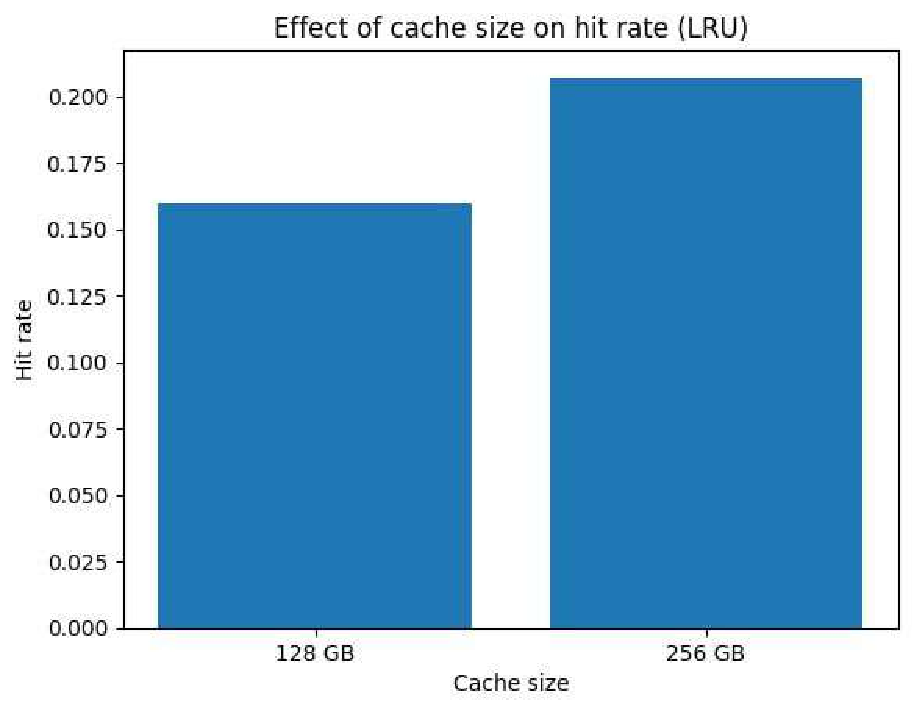
\includegraphics[width=\linewidth]{ablation_fig9_cache_size_hit_rate.pdf}
  \vspace{-25pt}
  \caption{Effect of cache size on hit rate (LRU).\\The difference between the cache 128GB and 256GB has a slight impact on the bandwidth of the clients, so it implies that bandwidth is not very sensitive to the size of the cache in this workload.}
  \label{fig:1-9}
\end{figure}

\noindent Figure \ref{fig:1-10} shows the middle eviction age in seconds for the same two cache sizes being talked about. As we can see that hen the cache is at 128 GB, objects are evicted around the 870s on the average, while at 256 GB the average eviction age increases to around 1280s. This shows that it is quite consistent with the hit rate trends. A larger cache holds objects longer, which increases the chance of reuse before eviction. It also indicates that the working set size of this trace is larger than 128 GB, so shrinking the cache forces the system to evict potentially useful objects much earlier. This larger retention window is also effective to stabilize DT to decrease the occurrence of misses to back-end during bursty periods.\\

\vspace{-15pt}
\begin{figure}[H]
  \centering
  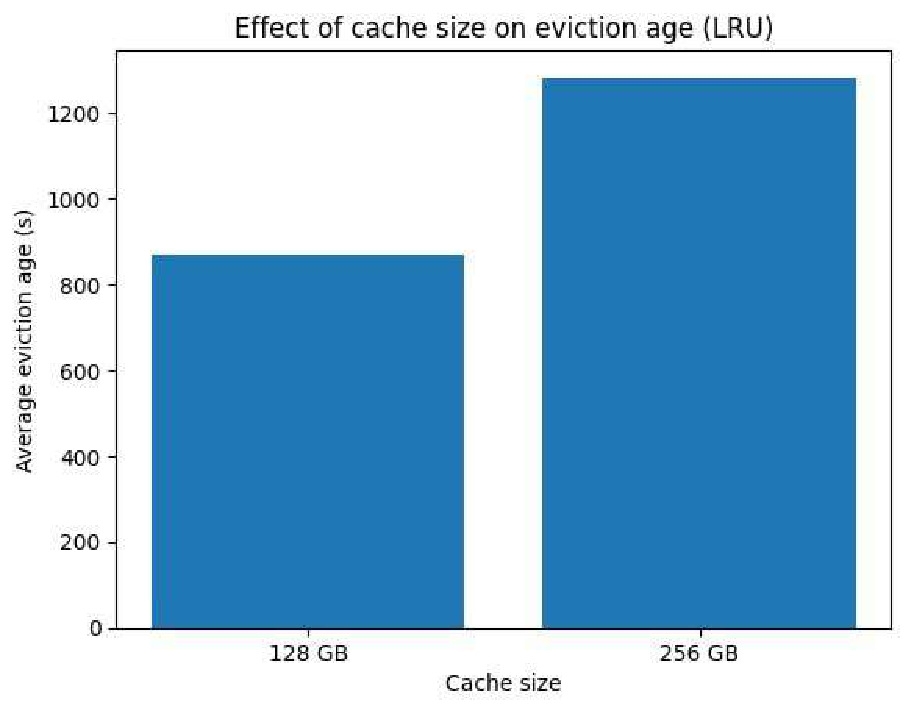
\includegraphics[width=\linewidth]{ablation_fig10_cache_size_eviction_age.pdf}
  \vspace{-25pt}
  \caption{Effect of cache size on eviction age (LRU).\\The cache with a 256 GB cache is significantly higher (compared to the 128 GB cache) in the number of chunk hits, which implies better locality coverage and a larger resident working set.}
  \label{fig:1-10}
\end{figure}

\noindent Figure \ref{fig:1-11} focuses on the IOPS saved ratio. Moving from 128 GB to 256 GB increases the fraction of backend I/O avoided by the cache. This aligns with the higher hit rate and longer eviction age. The key point here is that the gains are not only visible in logical hit rate, but also in the amount of physical backend work removed by caching.\\

\vspace{-15pt}
\begin{figure}[H]
  \centering
  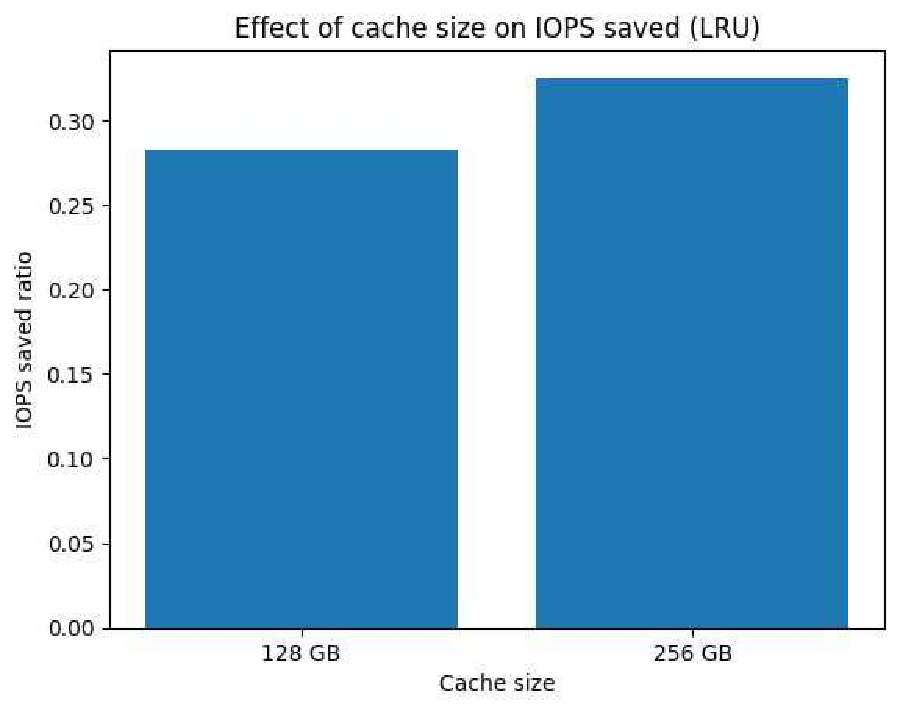
\includegraphics[width=\linewidth]{ablation_fig11_cache_size_iops_saved.pdf}
  \vspace{-25pt}
  \caption{Effect of cache size on IOPS saved ratio (LRU).\\There is a significant improvement in the hit rate between 128 GB to 256 GB as the higher the size of the cache the longer the reusable objects are kept in the cache.}
  \label{fig:1-11}
\end{figure}

\noindent Figure \ref{fig:1-12} looks at client bandwidth. Client throughput is already high for this trace, and the difference between 128 GB and 256 GB is small. Both configurations deliver similar MB/s to the client. This suggests that, for this particular workload and queueing regime, backend capacity is not the only bottleneck.\\

\vspace{-15pt}
\begin{figure}[H]
  \centering
  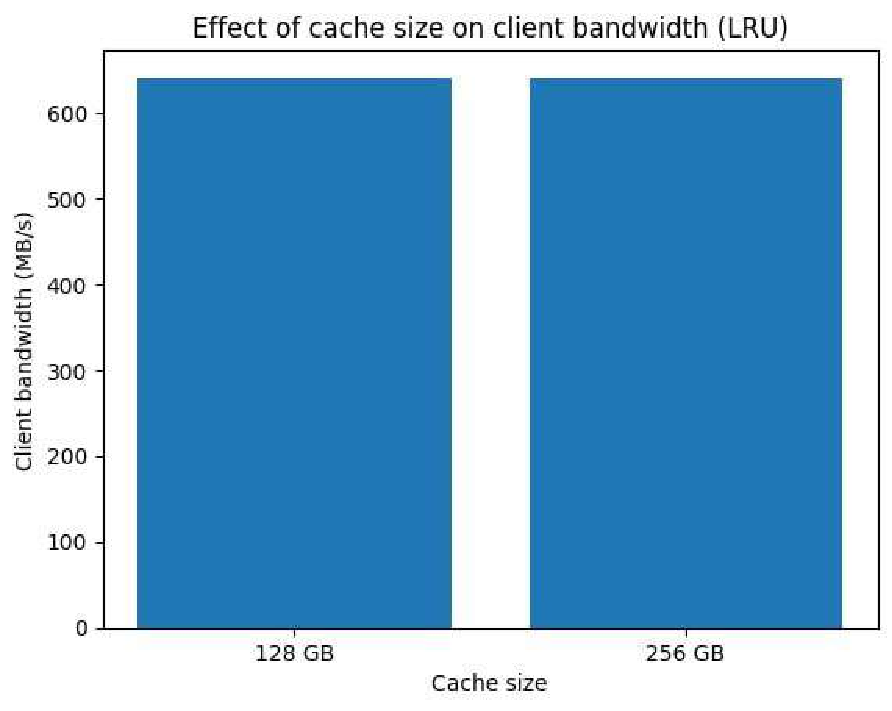
\includegraphics[width=\linewidth]{ablation_fig12_cache_size_client_bw.pdf}
  \vspace{-25pt}
  \caption{Effect of cache size on client bandwidth (LRU).\\The age of eviction increases significantly with a bigger cache and it demonstrates that objects are not evicted as quickly and have a higher chance of being reused.}
  \label{fig:1-12}
\end{figure}

\noindent Figure \ref{fig:1-13} examines flash write rate. Here the tradeoff becomes clear. The 256 GB configuration writes more MB/s to flash than the 128 GB configuration. The increase in flash writes is the price of the extra hits and IOPS savings we saw earlier. From an SSD endurance perspective, this means that while larger caches improve performance and stability, they also consume more write budget.\\

\vspace{-15pt}
\begin{figure}[H]
  \centering
  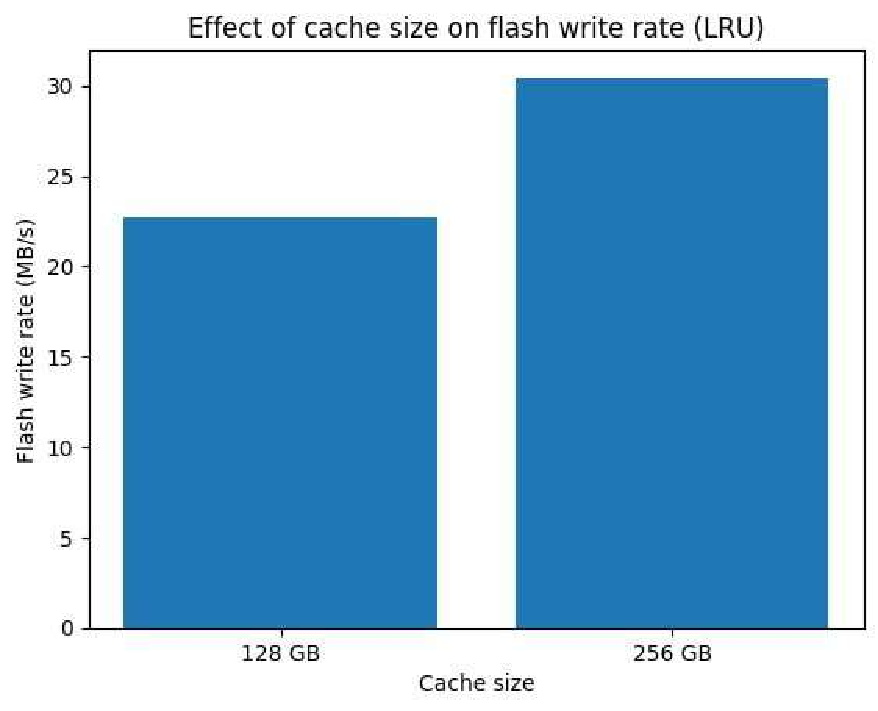
\includegraphics[width=\linewidth]{ablation_fig13_cache_size_flash_write.pdf}
  \vspace{-25pt}
  \caption{ Effect of cache size on flash write rate (LRU).\\The larger cache has a greater IOPS-reduced ratio, which proves to be offloaded by the back end better and does not depend on disk operations as much.}
  \label{fig:1-13}
\end{figure}

\noindent Figure \ref{fig:1-14} shows total chunk hits for the two cache sizes. The 256 GB cache serves substantially more chunk hits than the 128 GB cache, which again matches the hit rate and IOPS trends. The higher number of served chunks confirms that the additional capacity is being used to store genuinely useful data rather than just cold objects. When combined with the eviction-age results, this supports the idea that the working set comfortably fits within 256 GB but is constrained at 128 GB.\\

\vspace{-15pt}
\begin{figure}[H]
  \centering
  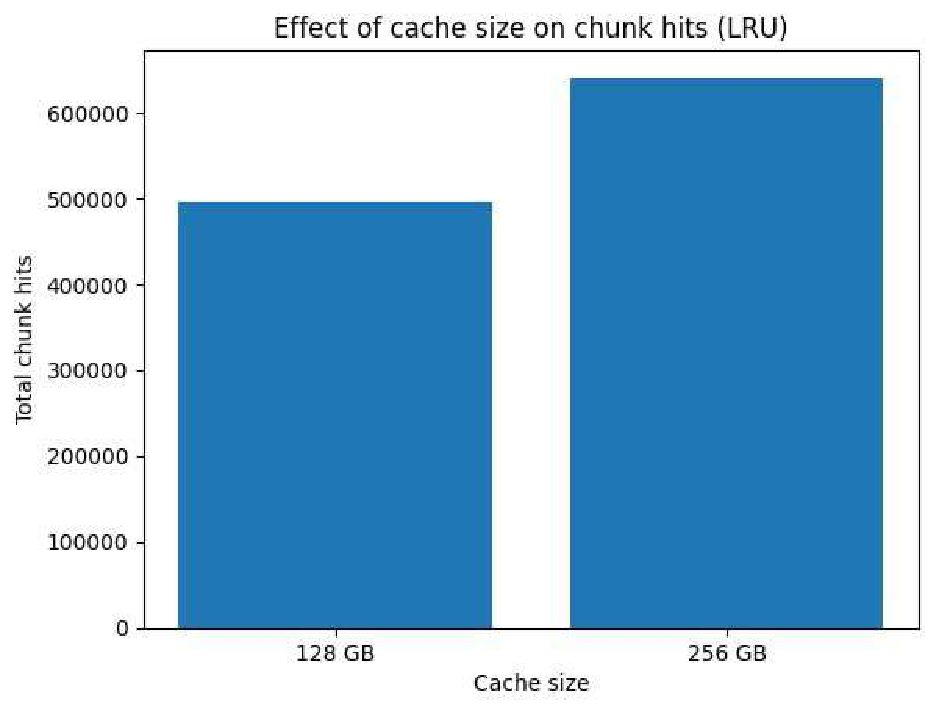
\includegraphics[width=\linewidth]{ablation_fig14_cache_size_chunk_hits.pdf}
  \vspace{-25pt}
  \caption{Effect of cache size on total chunk hits (LRU).\\The trade-off between performance gains and flash endurance is emphasized by expanding the cache because it boosts flash write rate by retaining objects longer and making it more write-intensive.}
  \label{fig:1-14}
\end{figure}

\noindent In general, the results from ablation shows consistency. So we can say the following will happen if we increase cache capacity from 128 GB to 256 GB will, improves hit rate and the IOPS saved ratio, increases the average eviction age and the number of chunk hits, has only a small effect on client bandwidth,
and raises the flash write rate. For this workload, 256 GB provides better backend offload and more stable DT behaviour, but at the cost of higher write traffic to the flash cache. In practice, this suggests that cache sizing for Baleen should consider both performance targets and flash endurance. If the deployment can tolerate the extra writes, the larger cache offers a more robust operating point, if flash lifetime is very tight, a smaller cache may be preferable even though it leaves some potential IOPS savings on the table.\\
\\Furthermore, the scaling behaviour manifested in the ablation indicates that the increments of capacity do not affect all the metrics in equal measure. Although the improvement in hit rate and DT stability can be observed, the marginal gains turn to decrease as the cache approaches the point when the majority of short-reuse objects have already been stored. This effect of diminishing returns implies that when the workload has a large number of long-reuse patterns then increasing capacity beyond that point offers minimal incremental value.

\clearpage
\section{Conclusion:}
\large The project provided a detailed analysis of the current policies of caching in the Baleen-FAST24 simulator with special emphasis on the dynamics of the combination of ML-guided admission, deadline-based eviction, and selective prefetching with respect to realistic tectonic traces. We find that all the mechanisms play a distinct part in the stability of the cache, and backend efficiency as well as the general hit rate, and that the highest performance improvements are only achieved upon combining all these components in a coordinated pipeline. We have experimented, conducted sensitivity analysis, and also ablation studies to observe that the moderation of the parameters always gives optimum trade-off between aggressiveness and stability, and this permits the system to be able to deal with the workload burstiness and phase shifts. The discussion also shows that the combination of learning-based filtering, temporally-aware eviction, and correlation-based prefetching can result in significant decreases in the I/O of backends as well as enhanced resilience when access patterns are varied. On the whole, this work has enhanced our insight into the interactions between the caching strategy in practice and the significance of the combined optimization of the admission, eviction and prefetching strategies towards the achievement of contemporary storage devices.

\clearpage
\bibliographystyle{ACM-Reference-Format}
\bibliography{refs}
\end{document}